%% The openany option is here just to remove the blank pages before a new chapter
\documentclass[a4paper]{article}


\usepackage{mystyle}
\addbibresource{refs.bib}


\usepackage{etoolbox}

\newtoggle{supervisor}
\toggletrue{supervisor}





\graphicspath{{figs/}}

\title{Mechanical Properties of Materials}
\pagenumbering{gobble}
\renewcommand{\familydefault}{\sfdefault}
\iftoggle{supervisor}{\newenvironment{annotation}{\color{red}}{}}{\newenvironment{annotation}{}{}}









\begin{document}

{\centering
{\Huge
IB Course B\\
Mechanical Properties of Materials\\}
\vspace{1cm}
{\LARGE
R.P. Thompson\\}

\vspace{3cm}
\begin{figure}[h!]
\centering
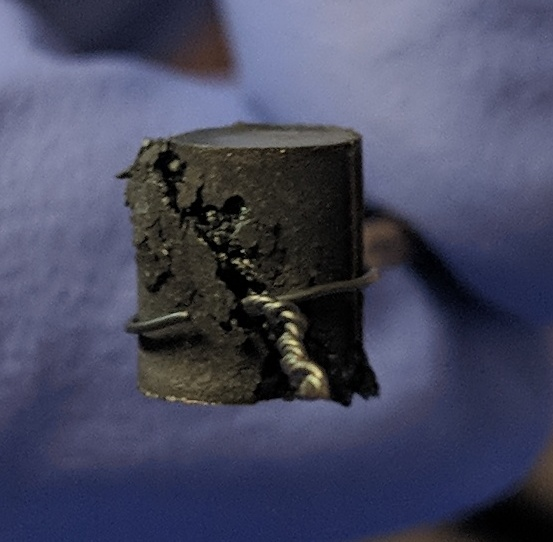
\includegraphics[width=0.5\textwidth]{crushed}
\end{figure}
}

\clearpage


\onehalfspacing
\section*{Introduction}

The mechanical behaviour of properties is one of the central themes of the subject. The properties that govern this behaviour are of direct interest for structural applications, indeed structural materials make up the vast majority of material use globally.

But even for materials that are used for their functional properties mechanical properties are important. The failure mode of many devices is mechanical in nature. Hence, regardless of the primary purpose of a material it is important that we understand the way that loading of structures leads to stresses and strains in a material, how to represent these quantities and the possible modes of failure that might arise as a result.

Building on Course E of IA, the course begins with the representation of stress and strain as tensors. The course will cover how structures can be loaded, particularly beams and struts. The last part of the course will develop the failure modes of materials, including fracture, fatigue, crushing, buckling and yielding.





\clearpage

\tableofcontents

\clearpage
\pagenumbering{arabic}


\section{Tensors}
\subsection{Revision of IA}

In IA the concept of normal and shear stresses were covered. Normal stresses and shear stresses can be defined with the equations:
\begin{equation*}
\sigma = \frac{\mathbf{F}}{A} \hspace{5cm}  \tau = \frac{\mathbf{F}}{A}
\end{equation*}
where the forces and areas are defined by:
\begin{figure}[h!]
\centering
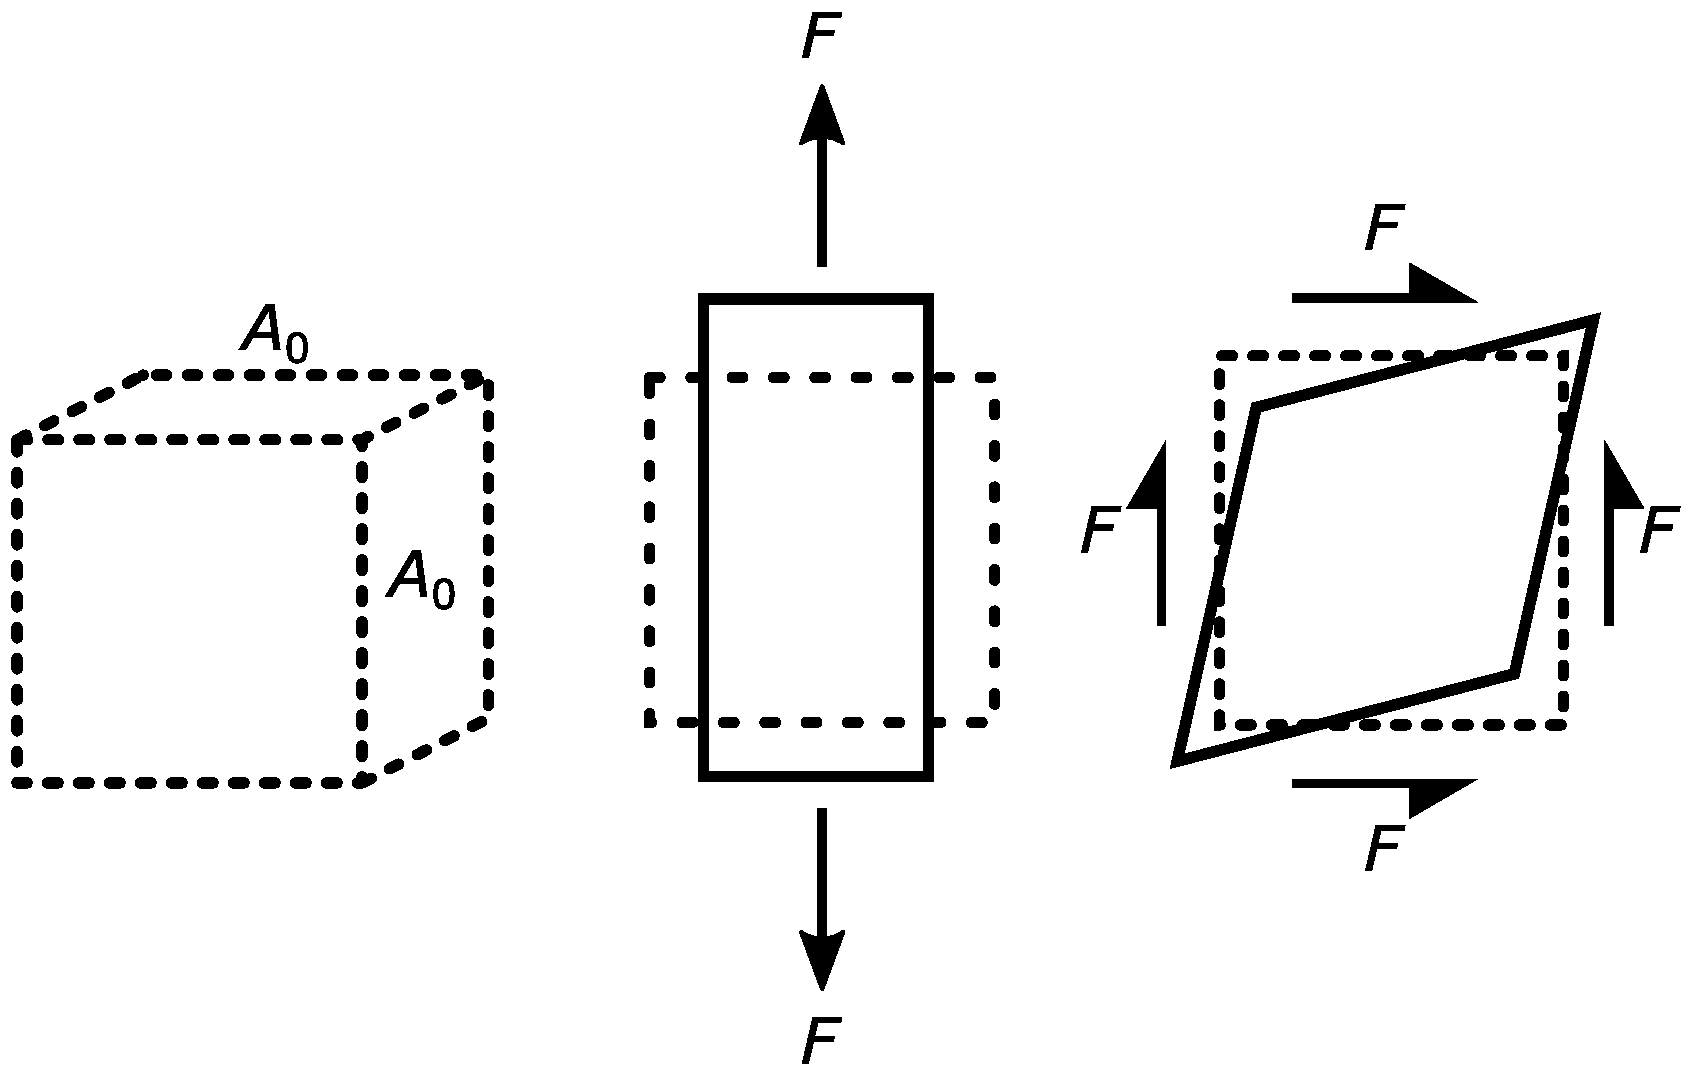
\includegraphics[width = 0.6\textwidth]{Stresses}
\end{figure}

The material will respond elastically as long as the stresses are below the failure stress, and we can define normal and shear strains:

\begin{equation*}
\varepsilon = \frac{\Delta x}{x_0} \hspace{5cm} \gamma = \frac{\Delta y}{x_0}
\end{equation*}
where the lengths are defined by:
\begin{figure}[h!]
\centering
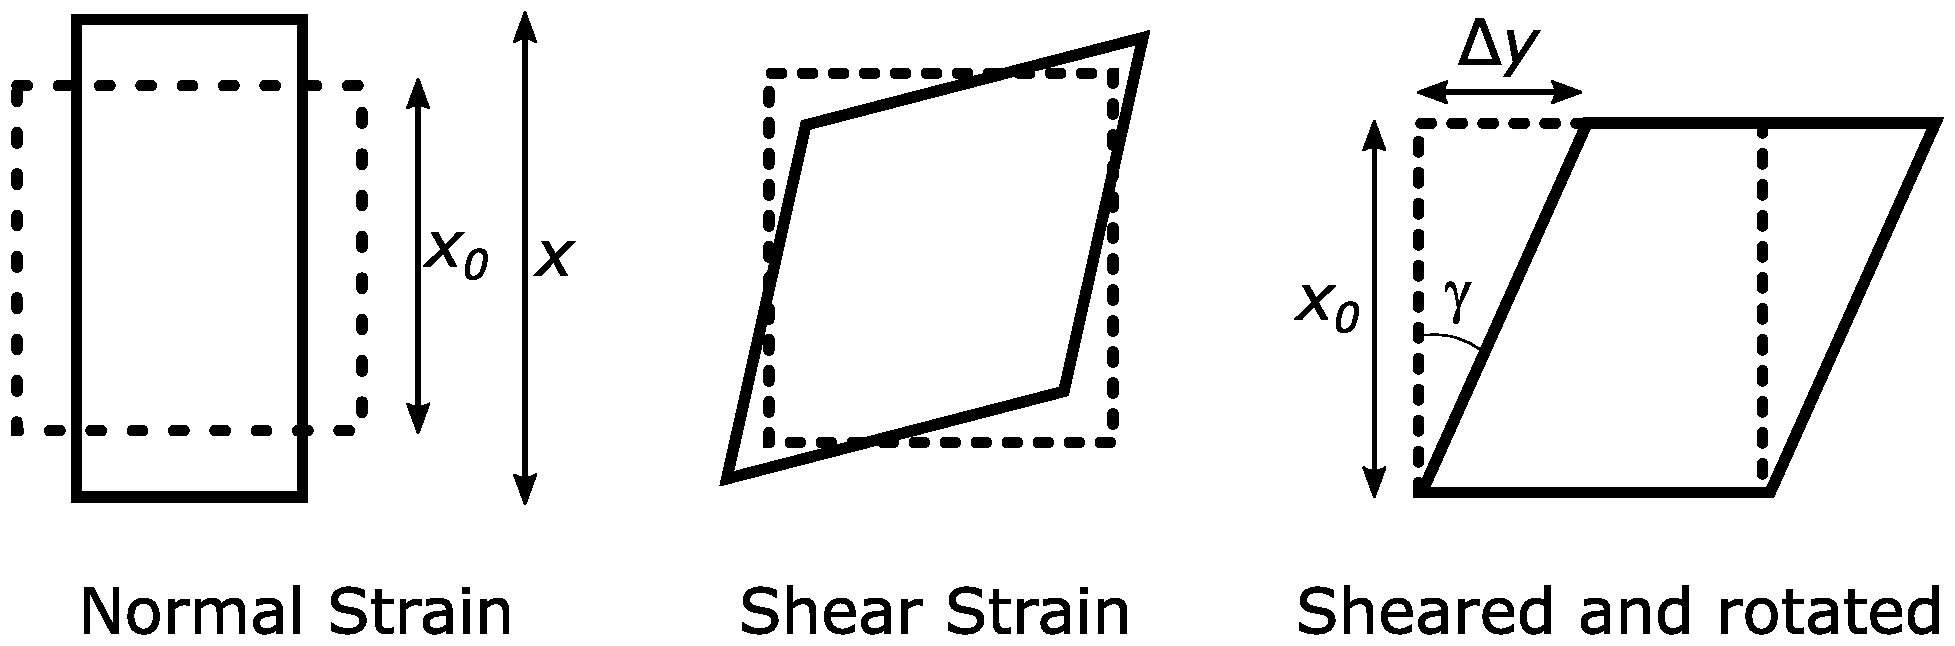
\includegraphics[width = 0.7\textwidth]{Strains}
\end{figure}

The quantities of stress and strain are linearly related for elastic behaviour and we can write:
\begin{align}
\sigma &= \varepsilon E \nonumber\\
\tau &= \gamma G \label{eqn:def_moduli}
\end{align}
where $E$ and $G$ are the Young's modulus and shear modulus respectively.

There are important points about this representation:
\begin{itemize}
\item For a general set of applied forces, both shear and normal stresses will develop, and furthermore the size of these components will vary as different sets of planes are considered, i.e.\ the frame of reference is important.
\item A stress or strain as defined above is implicitly defined by a magnitude and {\bf{two}} directions. For stress these are the direction that the force is acting in and the direction normal to the plane being considered. For strain these are the direction of displacement and the direction of the reference length.
\end{itemize}

Scalars and vectors are familiar concepts: scalars are defined by a magnitude, vectors are defined by magnitude and a single direction. Stress and strain cannot be completely described by scalars or vectors, and so cannot be resolved into components etc. Instead they can be described using tensors.


\subsection{Introduction to tensors}

A tensor is an $n$-dimensional array of values, where $n$ is the ``rank'' of the tensor. {\bf Scalars} and {\bf vectors} are \emph{zeroth} and \emph{first} rank tensors respectively. Properties that have no directionality and a single magnitude are scalars, and the concept of components does not apply.
\\
\\
\begin{annotation}
0\textsuperscript{th} rank tensors $\Longrightarrow$ Scalar quantities with no directionality.
\\
\\
Examples are temperature, density, energy, charge etc.
\end{annotation}
\\

A first rank tensor is a \emph{vector}. When represented as a tensor they have 3 values, or components, corresponding to the components in three mutually orthogonal directions. Each component can be thought of as having an index, usually written as a suffix. Several systems are used, such as \{$x,\,y,\,z$\} or \{$r,\,z,\,\theta$\}, here numerical suffices will be used: \{1,\,2,\,3\}. Vectors are then written
\begin{equation}
\mathbf{F} = F_i = [F_1,\, F_2,\, F_3]
\end{equation}
We will return to suffix notation, but the basic concept is as follows: wherever a suffix has a numerical value then the quantity refers to a specific component, e.g. $F_2$ is the magnitude of the component along the 2 axis, however where a suffix is a letter then this represents all the possible components, i.e. $F_i$ above is the  vector.
\\
\\
\begin{annotation}
1\textsuperscript{st} rank tensors $\Longrightarrow$ Vector quantities, a magnitude and direction and represented by a 1-D array with 3 components.
\\
\\
Examples are force, velocity, electric/magnetic field, polarisation, acceleration etc.
\end{annotation}

\subsubsection{Second rank tensors: Stress and Strain}

Stress and strain are examples of a second rank tensor, each component is defined in terms of two directions (e.g. the direction of the force and the normal of the plane upon which it acts defines a component of stress) and each component has two suffices, hence this is called a second rank tensor.
\\
\\
\begin{annotation}
2\textsuperscript{nd} rank tensors $\Longrightarrow$ tensors with a magnitude and two directions, represented by a 2-D array with 9 components. 
\\
\\
Examples are stress ($\sigma_{ij}$), strain ($\varepsilon_{ij}$), electrical resistivity ($\rho_{ij}$), thermal expansion coefficient ($\alpha_{ij}$) etc.
\end{annotation}

In each case the two suffices will have a physical interpretation. In the case of stress, the convention used here will be that the first suffix refers to the direction of the force being applied, and the second defines the normal of the plane upon which this force is acting (this convention can be reversed but as long as a single convention is used consistently then problems are unlikely). There are three directions in which a force or plane normal can lie, so there are nine combinations:

\begin{equation}
\sigma_{ij} = 
\begin{pmatrix}
\sigma_{11} & \sigma_{12} & \sigma_{13} \\
\sigma_{21} & \sigma_{22} & \sigma_{23} \\
\sigma_{31} & \sigma_{32} & \sigma_{33}
\end{pmatrix}\label{eqn:general_stress_tensor}
\end{equation}

For a component where $i$ and $j$ are equal, i.e. the main diagonal, the force acts perpendicular to the plane, and this component is a normal stress. Where $i$ and $j$ are not equal the force acts parallel to the plane and this component is a shear stress. For shear components the symbol $\tau_{ij}$ is sometimes used.
\\
\\


\begin{annotation}
$\sigma_{ii} \Longrightarrow $ Normal stress, force is parallel to plane normal

$\sigma_{ij} \Longrightarrow $ Shear stress, force is perpendicular to plane normal (sometimes written as $\tau_{ij}$)
\end{annotation}
\\
\\




\begin{figure}[bh!]
\centering
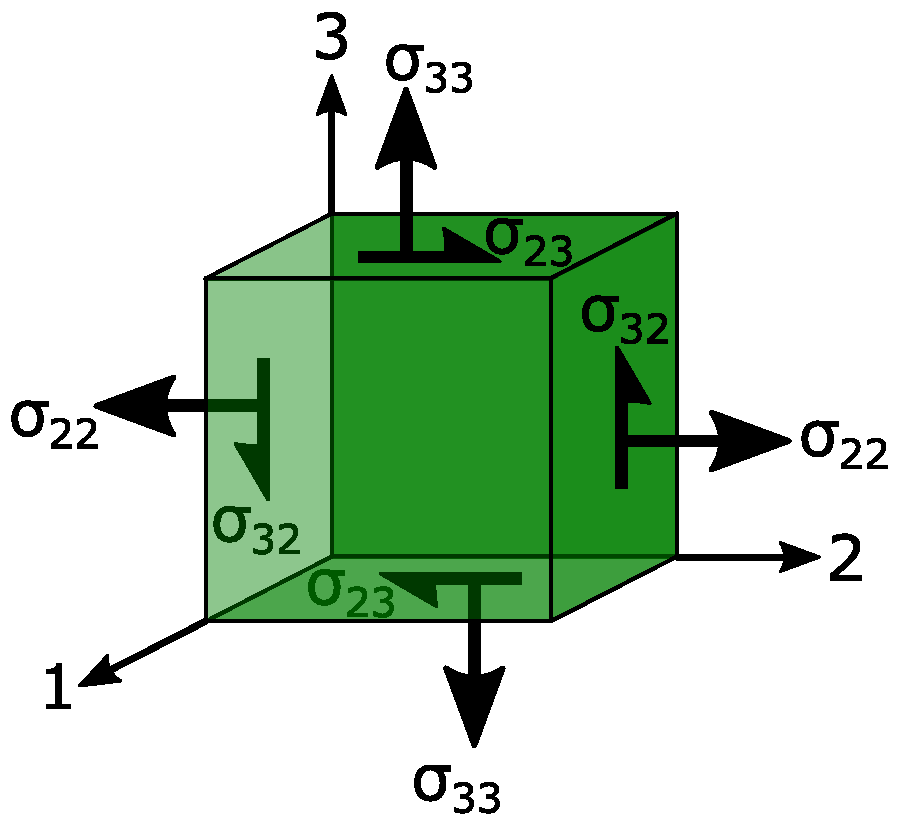
\includegraphics[width=0.66\textwidth]{Plane_Stress}
\caption{Illustration of the nomenclature of stresses acting on a body.\label{fig:plane_stress} }
\end{figure}

This nomenclature is shown for some of the possible stress components in \autoref{fig:plane_stress}. When thinking about stresses we assume that the body is in {\bf static equilibrium}, i.e. there are no net forces or moments acting on the body as a whole. 

This necessarily places constraints on the situation as depicted in \autoref{fig:plane_stress}. The simplest is that normal forces acting on opposite faces of the body must be equal, but for shear stresses there is a further constraint: not only must the forces on opposing faces be equal and opposite, e.g. the forces acting to give rise to $\sigma_{32}$, but also there must be a balance between the moments generated, such that $\sigma_{32} = \sigma_{23}$, preventing the rotation of the body under a net moment. This applies generally, so $\sigma_{ij} = \sigma_{ji}$, meaning that the stress tensor, \autoref{eqn:general_stress_tensor}, must be {\bf symmetrical}:
\\
\\

\begin{annotation}

\pgfdeclarelayer{background}
\pgfsetlayers{background,main}
{\centering
\begin{tikzpicture}
\centering
 \matrix[matrix of math nodes,left delimiter = (,right delimiter = ),row sep=10pt,column sep = 10pt] (m)
 {
\sigma_{11} & \sigma_{12} & \sigma_{13} \\
\sigma_{12} & \sigma_{22} & \sigma_{23} \\
\sigma_{13} & \sigma_{23} & \sigma_{33} \\
 };
\begin{pgfonlayer}{background}
 \draw[rounded corners,fill=green
,inner sep=3pt,fill opacity=0.3] (m-1-2.north west) -- (m-1-2.north east) -- (m-1-2.south east) -- (m-1-2.south west) -- (m-2-1.north east) -- (m-2-1.south east) -- (m-2-1.south west) -- (m-2-1.north west) -- (m-2-1.north east) -- (m-1-2.south west) -- cycle ;
 \draw[rounded corners,fill=green
,inner sep=3pt,fill opacity=0.3] (m-3-2.south east) -- (m-3-2.south west) -- (m-3-2.north west) -- (m-3-2.north east) -- (m-2-3.south west) -- (m-2-3.north west) -- (m-2-3.north east) -- (m-2-3.south east) -- (m-2-3.south west) -- (m-3-2.north east) -- cycle ;

 \draw[rounded corners,fill=green
,inner sep=3pt,fill opacity=0.3] (m-3-1.south east) -- (m-3-1.south west) -- (m-3-1.north west) -- (m-3-1.north east) -- (m-2-2.south west) -- (m-2-2.north west) -- (m-2-2.north east) -- (m-1-3.south west) -- (m-1-3.north west) -- (m-1-3.north east) -- (m-1-3.south east) -- (m-1-3.south west) -- (m-2-2.north east) -- (m-2-2.north west) -- (m-2-2.south west) -- (m-3-1.north east) -- cycle ;
\end{pgfonlayer}
\end{tikzpicture}
}

This means that only six components are required to fully define a stress state:

{\centering
\begin{tikzpicture}
\centering
 \matrix[matrix of math nodes,left delimiter = (,right delimiter = ),row sep=10pt,column sep = 10pt] (m)
 {
\sigma_{11} & \sigma_{12} & \sigma_{13} \\
\sigma_{12} & \sigma_{22} & \sigma_{23} \\
\sigma_{13} & \sigma_{23} & \sigma_{33} \\
 };
\begin{pgfonlayer}{background}
 \node[inner sep=3pt,fit=(m-1-1)]          (1)   {};
 \node[inner sep=3pt,fit=(m-1-2) (m-2-3)]  (2)   {};
 \node[inner sep=3pt,fit=(m-3-3)]          (3)   {};
 \draw[rounded corners,fill=green
,inner sep=3pt,fill opacity=0.3] (1.north west) -- (2.north east) |- (3.south west) |- (2.south west) |- (1.south west) -- cycle;
\end{pgfonlayer}
\end{tikzpicture}
}



BUT values depend on the reference axes.
\\
\\

\end{annotation}

\subsubsection{Axis Transformation}


There are six independent components of a general stress state, 3 normal stresses and 3 shear stresses. While the stress state itself must be unaffected by the choice of axes, the magnitude of these components will be affected, in much the same way as vectors. In fact, any tensor can be {\bf transformed} to refer to a new set of axes if the orientation relationship between the new set and old set of axes is known. 


The idea that the components of shear and normal stress vary with reference frame is not too difficult to understand. In \autoref{fig:shear_normal} it can be seen that two equal and perpendicular shear stresses in one frame of reference can be thought of as two equal and perpendicular normal stresses if the reference frame is rotated by \SI{45}{\degree}.


\begin{figure}[h!]
\centering
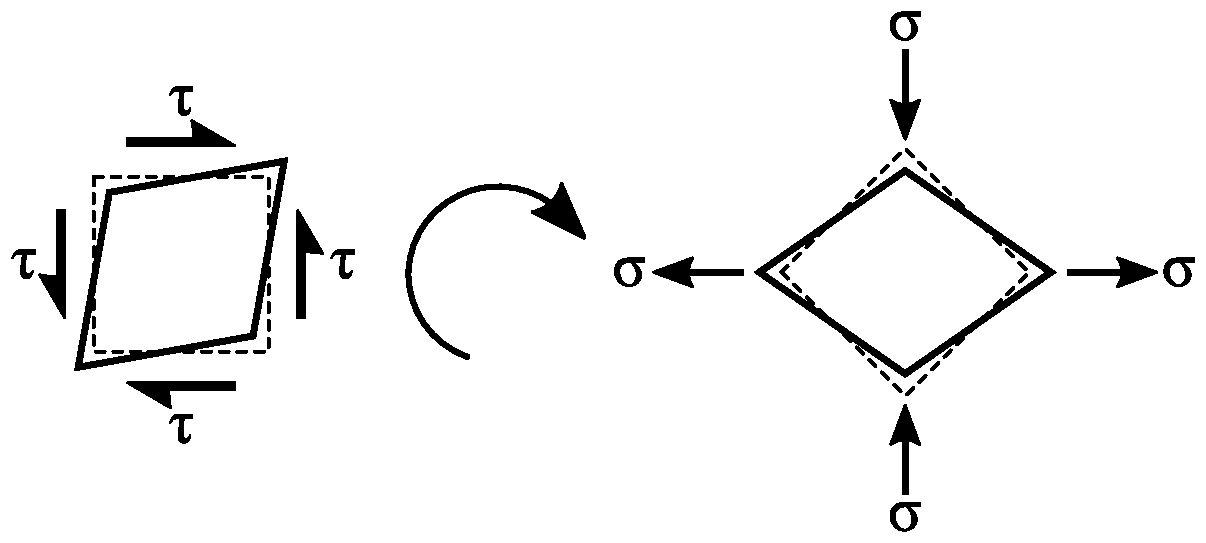
\includegraphics[width=0.6\textwidth]{shear_normal_equivalence}
\caption{Illustration that a pure shear stress state in one frame of reference can be represented by normal stresses in another.\label{fig:shear_normal}}
\end{figure}


This concept was partially discussed in IA course E when discussing slip systems and the resolved shear stresses.

\subsubsection*{Recap of Schmid Factor - See IA course E}


\begin{figure}[h!]
\centering
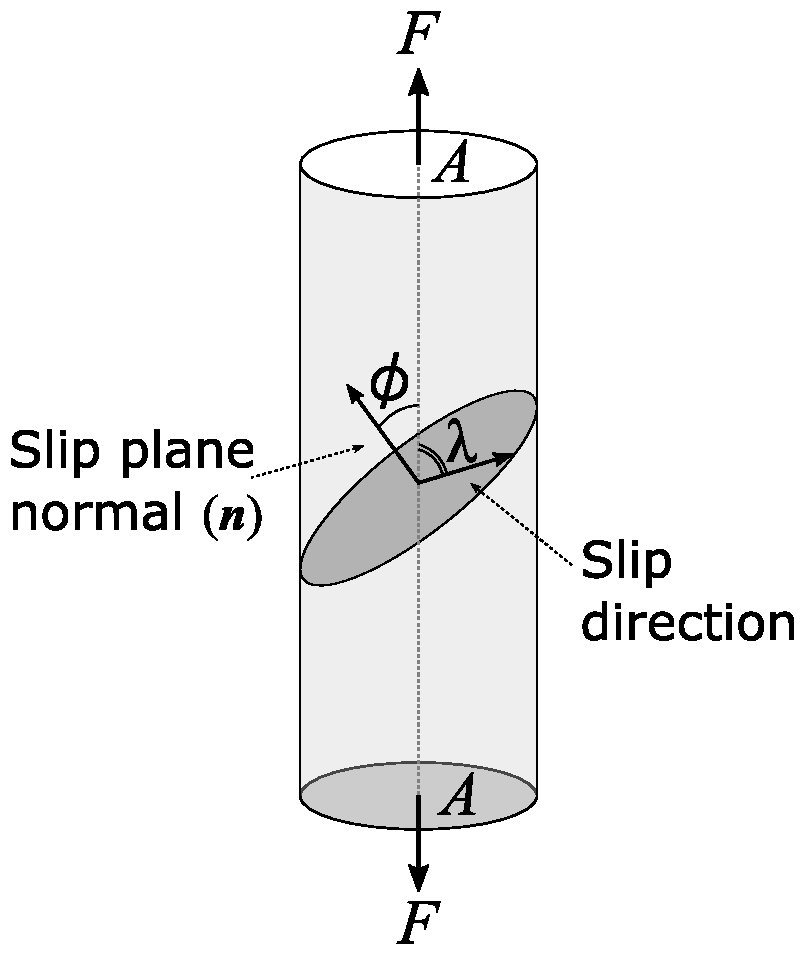
\includegraphics[width = 0.5\textwidth]{Schmid_Factor}
\caption{The geometry of the Schmid factor\label{fig:schmid_factor}}
\end{figure}

The Schmid factor is a method for calculating the shear component relevant to a particular slip system, i.e. the force acting along the slip direction and acting on the slip plane under the influence of a single applied tensile force.

By considering the slip system depicted in \autoref{fig:schmid_factor}, the component of the force parallel to the slip direction is $F\cos\lambda$, and the area of the plane is $A/\!\cos\phi$

This gives the resolved shear stress as:

\begin{equation}
\tau_\text{R} = \frac{F}{A} \cos \phi \cos \lambda \label{eqn:Schmid}
\end{equation}



The idea that the orientation being considered will affect the balance of normal can be intuitively understood

\FloatBarrier

Given a set of reference axes, \{1, 2, 3\}, a vector, $\mathbf{F}$, can be expressed as three components along each of these axes, $[F_1,\, F_2,\, F_3]$. If some other set of axes is defined, \{1', 2', 3'\}, then there will another representation of the vector  $\mathbf{F} = [F_{1'},\, F_{2'},\, F_{3'}]$. In \autoref{fig:axes_rotation} a vector is shown with respect to two axis sets that are related to each other by a rotation of $\phi$ about the 3 axis (which, therefore, coincides with the 3' axis).



\begin{figure}[h!]
\centering
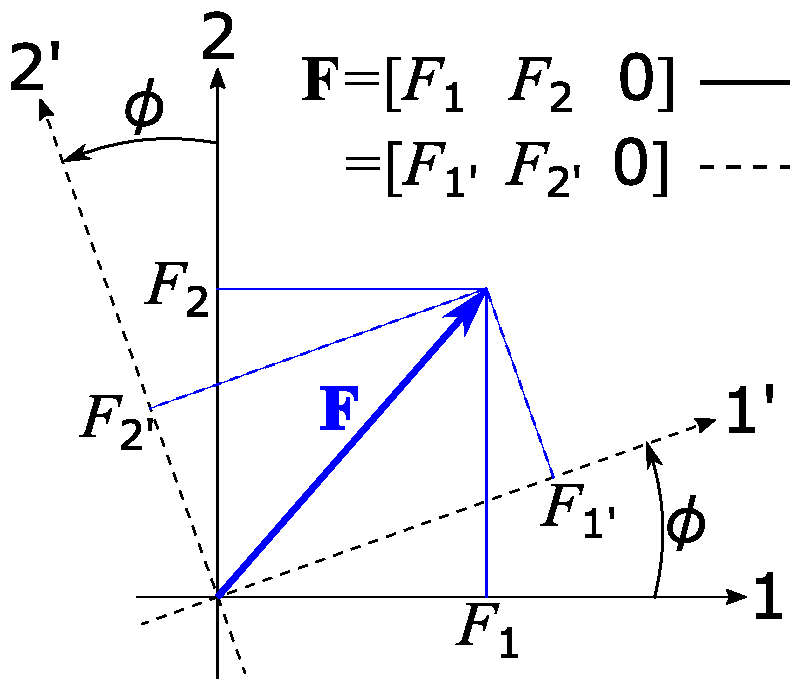
\includegraphics[width=0.6\textwidth]{rotate_axes}
\caption{Rotation, about the $3$ axis, of the axes defining the reference frame of a vector $\mathbf{F}$.\label{fig:axes_rotation}}
\end{figure}


The values of $F_{1'}$ and $F_{2'}$ can be found by resolving the components of $\mathbf{F}$, $F_2$ and $F_3$, along the 1' and 2' axes:

\begin{align}
F_{1'} &= F_1 \cos(1' \angle 1) + F_2 \cos(2' \angle 1) \nonumber\\
F_{2'} &= F_1  \cos(2' \angle 1) + F_2 \cos(2' \angle 2)
\end{align}

where the notation $(i' \angle j)$ indicates the angle between the $i'$ and $j$ axes.

In terms of $\phi$ this can be written:

\begin{align}
F_{1'} &= F_1 \cos(\phi) + F_2 \sin(\phi) \nonumber\\
F_{2'} &= - F_1  \sin(\phi) + F_2 \cos(\phi)
\end{align}

These trigonometric functions are key to transforming axes, and we can formulate a more general solution, known as direction cosines, the cosine of the angle from the new axis, $i'$, to the old axis, $j$:
\begin{annotation}
$$
a_{ij} = \cos(i' \angle j)
$$
\end{annotation}

This notation allows for rotation to be generalised to three dimensions:

\begin{align}
F_{1'}  &= a_{11}F_1 + a_{12} F_2 + a_{13} F_3 \nonumber\\
F_{2'}  &= a_{21}F_2 + a_{22} F_2 + a_{23} F_3 \\
F_{3'} &= a_{31}F_1 + a_{32} F_2 + a_{33} F_3 \nonumber
\end{align}

This can be written as a matrix operation:

\begin{equation}
\begin{bmatrix}
F_{1'} \\
F_{2'} \\
F_{3'}
\end{bmatrix} = 
\begin{bmatrix}
T
\end{bmatrix}
\begin{bmatrix}
F_1 \\ F_2 \\ F_3
\end{bmatrix}
\end{equation}
where the transformation matrix, $\begin{bmatrix}
T
\end{bmatrix}$, is given by:
\begin{equation}
\begin{bmatrix}
T
\end{bmatrix}
= \begin{bmatrix}
a_{11} & a_{12} & a_{13} \\
a_{21} & a_{22} & a_{23} \\
a_{31} & a_{32} & a_{33}
\end{bmatrix}
\end{equation}

For the transformation illustrated in \autoref{fig:axes_rotation} the transformation matrix would be:

\begin{equation}
\begin{bmatrix}
T
\end{bmatrix}
= \begin{bmatrix}
1 & 0 & 0 \\
0 & \cos\phi & \sin\phi \\
0 & -\sin\phi & \cos \phi
\end{bmatrix}
\end{equation}


This transformation matrix is similar to some you may have seen before when studying matrices in maths in previous years. You may notice that the sign of some of the terms is the opposite of what you expect, this is because we are rotating the reference frame, rather than the vector, effectively reversing the sign of the angle.

\subsubsection{Einstein summation convention}

These sorts of equations can be written more concisely, and more generally for higher order tensors, using the {\bf Einstein summation convention}. Whenever an index is repeated within a single term in an equation then a summation over all values of that index should be performed. Matrix multiplication provides a good example:

\begin{equation}
C_{ik} = A_{ij} B{jk} =  \sum_j A_{ij} B{jk} 
\end{equation}

where $j$ is a dummy suffix, i.e. it occurs twice in the term on the right hand side, and so we sum over all the possible values of $j=1,2,3$:

\begin{annotation}
\begin{equation}
C_{ik} = A_{i1}B_{1k} + A_{i2}B_{2k} + A_{i3}B_{3k}
\end{equation}
\end{annotation}


The example of a rotation above can be written:

\begin{equation}
F_{i'} = a_{ij}F_j
\end{equation}
\begin{annotation}
\centering
$j$ occurs twice
\end{annotation}

i.e. the first component of the force with respect to the new axes is:
\begin{equation}
F_{1'} = a_{11}F_1 + a_{12}F_2 + a_{13}F_3
\end{equation}
and so on for the other two components.
\\
\begin{annotation}
\begin{align*}
F_{2'} &= a_{21}F_1 + a_{22}F_2 + a_{23}F_3 \\
F_{3'} &= a_{31}F_1 + a_{32}F_2 + a_{33}F_3
\end{align*}
\end{annotation}
\\

To simplify the nomenclature this is often written with the prime on the symbol rather than the suffix to denote the transformed version:
\begin{equation}
F'_i = a_{ij}F_{j}
\end{equation}


This generalises to higher order tensors in a relatively straightforward manner:

\begin{equation}
\sigma'_{ij} = a_{ik} a_{jl} \sigma_{kl}
\end{equation}
\begin{annotation}
Apply the Einstein summation convention to $k$ and $l$
\end{annotation}
\\
\\

To illustrate this we can write the full equation for the $i=1$, $j=1$ component of $\sigma'_{ij}$:

\begin{align}
\sigma'_{11} =\,\,\, &a_{11}a_{11}\sigma_{11} + a_{11}a_{12}\sigma_{12} + a_{11}a_{13}\sigma_{13} \nonumber\\
 &a_{12}a_{11}\sigma_{21} + a_{12}a_{12}\sigma_{22} + a_{12}a_{13}\sigma_{23} \\
 &a_{13}a_{11}\sigma_{31} + a_{12}a_{13}\sigma_{23} + a_{13}a_{13}\sigma_{33} \nonumber
\end{align}



\begin{annotation}
Similarly for the 2-3 component:

\begin{align}
\sigma'_{23} =\,\,\, &a_{21}a_{31}\sigma_{11} + a_{21}a_{32}\sigma_{12} + a_{21}a_{33}\sigma_{13} \nonumber\\
                     &a_{22}a_{31}\sigma_{21} + a_{22}a_{32}\sigma_{22} + a_{22}a_{33}\sigma_{23} \nonumber \\
                     &a_{23}a_{31}\sigma_{31} + a_{22}a_{33}\sigma_{23} + a_{23}a_{33}\sigma_{33} \nonumber
\end{align}
And so on for the other components. c.f. Schmid law, \autoref{eqn:Schmid}, the shear is related to the normal stress by two direction cosines.

$$
\tau = \cos\phi \cos\lambda \sigma
$$
$$
\sigma_{23} = a_{21} a_{31} \sigma_{11}
$$

End of Lecture 1!
\end{annotation}
\\

\subsubsection{Principal stresses and strains, and the Secular Equation}

Using the transformations described above we can change a tensor to refer to new axes and change the values of the different components. Using this we can identify {\bf Principal Stresses }. These are normal stresses that act on {\bf Principal Planes}, which, by definition, have no shear stress acting upon them. A stress state expressed as principal stresses has the form:

\begin{equation}
\sigma_{ij} = \begin{annotation}
\begin{bmatrix}
\sigma_1 & 0 & 0 \\
0 & \sigma_2 & 0 \\
0 & 0 & \sigma_3
\end{bmatrix}\qquad
\text{where}\, \sigma_1,\,\, \sigma_2 \,\,\text{and}\,\, \sigma_3 \text{ are principal stresses}
\end{annotation}
\end{equation}

These are also the eigenvalues of the tensor. The single suffix is used to denote the fact that these are principal stresses. Obtaining the principal stresses is equivalent to diagonalising the tensor.

Second rank tensors are diagonalised in the same way as matrices, by solving the {\bf secular equation} (see a mathematics textbook for the derivation):

\begin{align}
\left|\sigma_{ij} - \lambda \mathbf{I} \right| = 0\qquad \begin{annotation}
\text{where {\bf I} is a unit matrix}
\end{annotation} \nonumber\\
\left| \begin{matrix}
\sigma_{11} - \lambda & \sigma_{12} & \sigma_{13} \\
\sigma_{21} & \sigma_{22} - \lambda & \sigma_{23} \\
\sigma_{31} & \sigma_{32} & \sigma_{33} - \lambda
\end{matrix}\right| = 0 \label{eqn:secular_equation}
\end{align}

To solve this equation we must use the determinant of a matrix:
\\

\begin{annotation}
$2 \times 2$
$$
A = \begin{bmatrix}
a & b \\
c & d
\end{bmatrix} \qquad \qquad \text{det} A = |A| = ad - bc
$$

$3\times3$

$$
|A| = \left| \begin{matrix}
a & b & c \\
d & e & f \\
g & h & i
\end{matrix} 
\right| = a \left| 
\begin{matrix} 
e & f \\ h & i\end{matrix} \right|
- b \left| 
\begin{matrix} 
d & f \\ g & i\end{matrix} \right|
+ c \left| 
\begin{matrix}
d & e \\
g & h
\end{matrix}
\right|
$$
\end{annotation}



For equation~\ref{eqn:secular_equation}, this gives a cubic equation for $\lambda$, each root of which is a principle stress. Using the determinant the secular equation becomes:

\begin{equation}
(\sigma_{11} - \lambda)[(\sigma_{22} - \lambda)(\sigma_{33}-\lambda) - \sigma_{23}^2] - \sigma_{12}[\sigma_{12}(\sigma_{33}-\lambda)-\sigma_{23}\sigma_{13}] + \sigma_{13}[\sigma_{12}\sigma_{13} - (\sigma_{22}-\lambda)\sigma_{13}] = 0
\end{equation}
This can be written:
\begin{equation}
\lambda^3 - I_1 \lambda^2 + I_2 \lambda - I_3 = 0 \label{eqn:cubic_roots}
\end{equation}
where
\begin{align}
I_1 &= \sigma_{11} + \sigma_{22} + \sigma_{33} \nonumber \\
I_2 &= \sigma_{11} \sigma_{22} + \sigma_{22} \sigma_{33} + \sigma_{33} \sigma_{11} - \sigma_{12}^2 - \sigma_{23}^2 - \sigma_{31}^2 \\
I_3 &= \sigma_{11}\sigma_{22}\sigma_{33} + 2\sigma_{12}\sigma_{23}\sigma_{31} - \sigma_{11} \sigma_{23}^2 - \sigma_{22}\sigma_{13}^2 - \sigma_{33}\sigma_{12}^2 \nonumber
\end{align}

These coefficients are called the invariants of the stress (or any other) tensor. They are not changed by a transformation of axes. A general stress state requires solving the cubic equation~\ref{eqn:cubic_roots}, though often things are simplified if one of the principle stress is already know, as this reduces the problem to a two-dimensional one.



\subsection{Mohr's Circle}

While finding the principal stresses by solving the secular equation is straightforward (if tedious), most problems involving stress states are not likely to be so generalised. It is quite common to know the magnitude and orientation of one principal stress and the corresponding plane, but to have more interest in principal directions within that plane, perhaps in how the normal and shear stresses vary with orientation within that plane.

If this is the case, and one root of the cubic secular equation is known then the problem reduces to a quadratic equation which can be solved via a geometrical construction, called Mohr's circle, which dates back to 1892 and was proposed by the German civil engineer Christian Otto Mohr.

If the 1-2 plane is a principal plane (i.e.\ $\sigma_{33}$ is a principal stress, and therefore $\sigma_{13} = \sigma_{23} = 0$) then the secular equation becomes:
\begin{equation}
\left| \begin{matrix}
\sigma_{11} - \lambda & \sigma_{12} & 0 \\
\sigma_{12} & \sigma_{22} - \lambda & 0 \\
0 & 0 & \sigma_{33}-\lambda
\end{matrix}\right| = 0
\end{equation}
remembering that $\sigma_{ij} = \sigma_{ji}$.

This becomes:
\begin{align}
(\sigma_{33}- \lambda)[(\sigma_{11} - \lambda)(\sigma_{22} - \lambda) - \sigma_{12}^2] = 0 \nonumber \\
\implies \lambda^2 - (\sigma_{11} + \sigma_{22})\lambda + (\sigma_{11}\sigma_{22} - \sigma_{12}^2) = 0
\end{align}

If we denote the two roots of this equation $\sigma_1$ and $\sigma_2$, we can write the solution as:

\begin{equation}
\sigma_1, \sigma_2 = \left( \frac{\sigma_{11} + \sigma_{22}}{2} \right) \pm \,\sqrt[]{\left( \frac{\sigma{11}-\sigma_{22}}{2}\right)^2 + \sigma_{12}^2} \label{eqn:Mohrs_circle_equation}
\end{equation}

The form of equation~\ref{eqn:Mohrs_circle_equation} can be interpreted graphically, where the first term defines the circles centre and the second term defines the radius. The circle would then be plotted with normal stresses along the horizontal axis and shear strains along the vertical axis.

\begin{figure}[hb!]
\centering
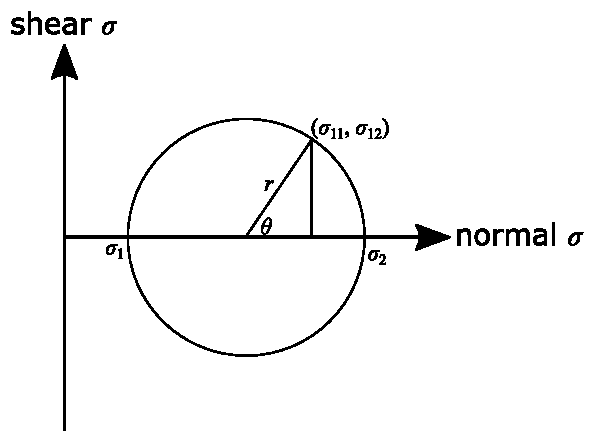
\includegraphics[width=0.5\textwidth]{Mohrs_Circle}
\caption{The graphical representation of the variation in normal and shear stresses as the frame of reference is rotated about a perpendicular principal axis.}
\end{figure}

\begin{annotation}
From this we can say:
\begin{equation}
r = \sqrt[]{\left( \frac{\sigma{11}-\sigma_{22}}{2}\right)^2 + \sigma_{12}^2} \qquad \qquad \tan \theta = \frac{2\sigma_{12}}{\sigma_{11} - \sigma_{22}}
\end{equation}
\end{annotation}

These results are derivable from the general transformation of tensors:
\begin{equation}
\sigma_{ij}' = a_{ik}a_{jl}\sigma_{kl}
\end{equation}
Since the 3 axis is a principal axis, we know $\sigma_{3}$ is a principal stress, and $\sigma_{13}=\sigma_{31}=0$ and $\sigma_{23}=\sigma_{32}=0$, this is simpler than the general case. If the transformation is:

\begin{equation}
a_{ij} = \left[ \begin{matrix}
\cos\phi & \sin\phi & 0 \\
-\sin\phi & \cos\phi & 0  \\
0 & 0 & 1
\end{matrix} \right]
\end{equation}
then the stresses are given by:
\begin{align}
\sigma_{11}' &= \cos^2\phi \sigma_1 + \sin^2\phi \sigma_2 \nonumber \\
\sigma_{22}' &= \sin^2\phi \sigma_1 + \cos^2\phi \sigma_2 \\
\sigma_{12}' &= - \sin\phi\cos\phi \sigma_1 + \sin \phi \cos \phi \sigma_2 \nonumber
\end{align}


These can be rearranged using trigonometric identities to be in terms of $2\phi$:

\begin{align}
\sigma_{11}' &= \left(\frac{\sigma_1 + \sigma_2}{2} \right) + \left( \frac{\sigma_1 - \sigma_2}{2} \right)\cos 2\phi \nonumber \\
\sigma_{22}' &= \left( \frac{\sigma_1 + \sigma_2}{2} \right) - \left( \frac{\sigma_1 - \sigma_2}{2} \right)\cos 2 \phi \\
\sigma_{12}' &= - \left( \frac{\sigma_1 - \sigma_2}{2}\right) \sin 2\phi
\end{align}

These equations can be solved with the circle construction above, where $2\phi = \theta$. The stress components (normal and shear) are given by the coordinates of a point on the circumference of the circle. As the frame of reference is rotated by an angle $\phi$, the point rotates around the circumference of the circle by an angle of $2\phi$. The circle is defined by the two principal stresses in question (here $\sigma_1$ and $\sigma_2$, the centre lies at the mean of the two principal stresses and the radius is half of the difference between the two principal stresses.

\begin{figure}[h!]
    \centering
    \begin{subfigure}{0.45\textwidth}
        \centering
        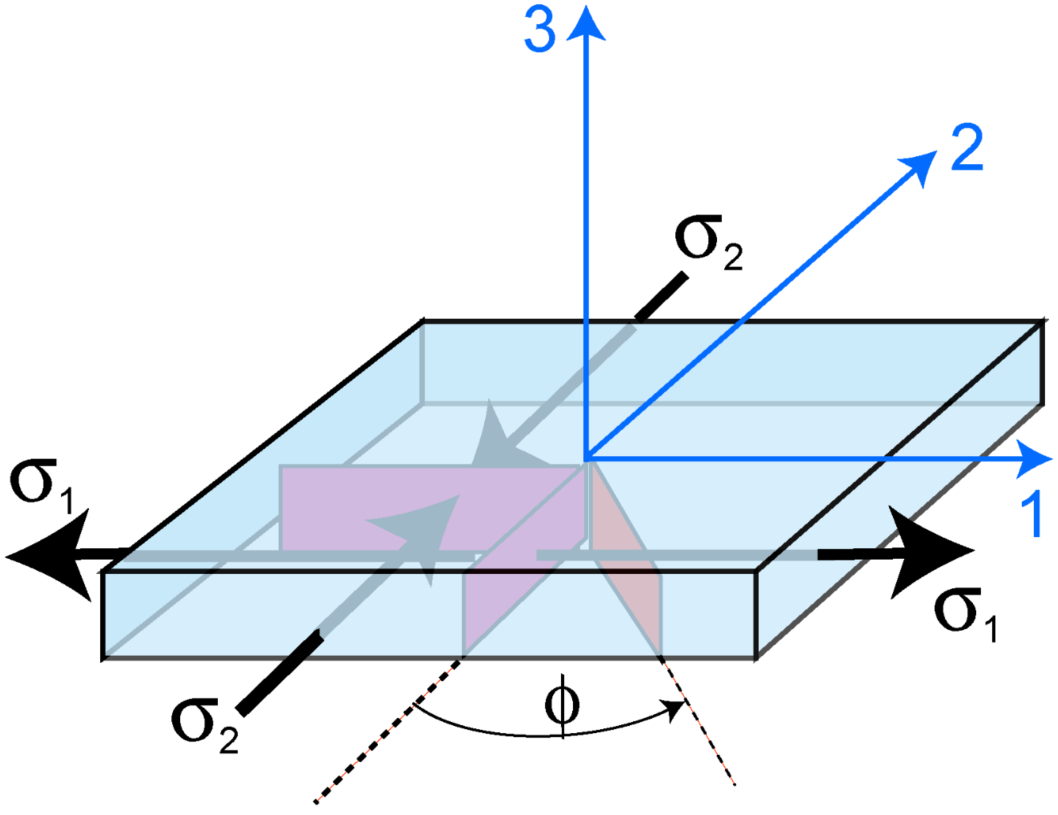
\includegraphics[width=\textwidth]{Real_space_rotate}
        \caption{}
    \end{subfigure}
~
    \begin{subfigure}{0.45\textwidth}
        \centering
        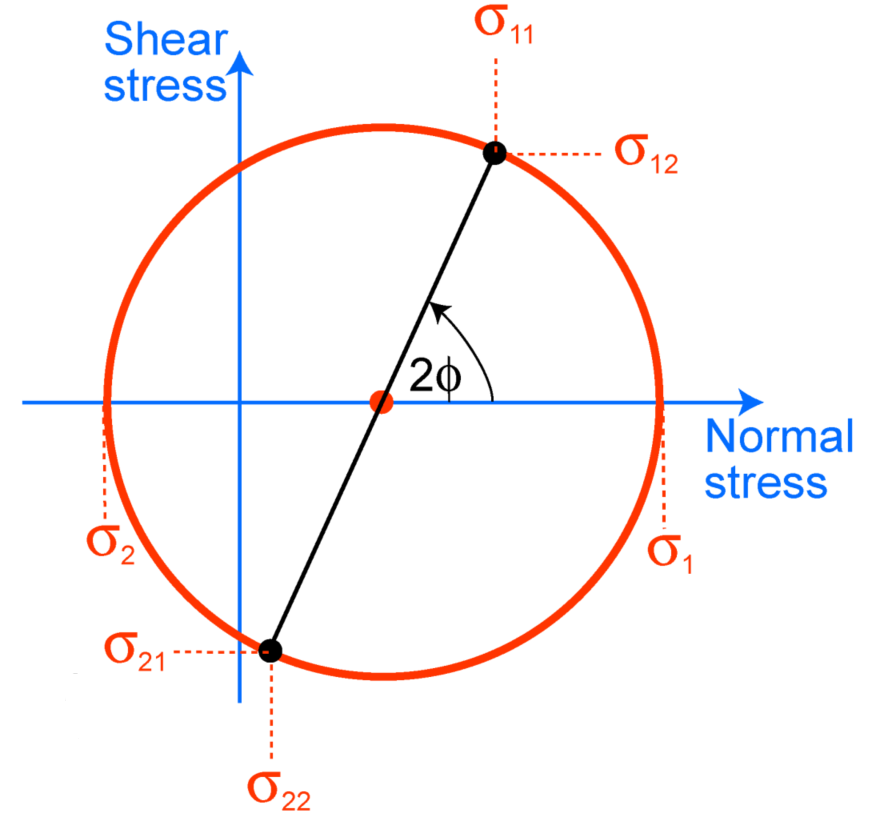
\includegraphics[width=\textwidth]{mohrs_circle_rotate}
        \caption{}
    \end{subfigure}
    \caption{Starting from a frame of reference where all the stresses are principal, i.e.\ a tension parallel to the 1-axis, a compression parallel to the 2-axis and no stress parallel to the 3-axis (a), the Mohr's circle construction allows us to calculate the stress components (both normal and shear) as the frame of reference is rotated. Note that this relies on the assumption that the 3 direction is a principal direction or equivalently that $\sigma_3$ is a principal stress.
    }
\end{figure}


\begin{annotation}
Conventions:
\begin{itemize}
\item Tensile stresses (normal by definition) are positive.
\item Compressive stresses (also normal) are negative.
\item There is no physical meaning to the sign of a shear stress, but clearly can \emph{change} sense if a force is reversed.
\end{itemize}
\end{annotation}



\subsubsection{Constructing Mohr's Circle}

Mohr's circle is a convenient graphical representation of the transformation of rotating the frame of reference about a principal axis. It allows the determination of various useful quantities including the principal stresses, the maximum shear stress, or the particular normal and shear components at arbitrary orientations. One common use is to find the principal stresses, $\sigma_1$ and $\sigma_2$, given the values of $\sigma_{11}$, $\sigma_{22}$ and $\sigma_{12}$ in some other frame of reference.

\begin{itemize}
\item First, construct a graph with normal stress along the horizontal axis and shear stress along the vertical axis using the same scale for both. The convention is that positive shear is downwards, and positive normal stress point to the right.

\item Plot the points ($\sigma_{11}$, $-\sigma_{12}$) and ($\sigma_{22}$, $\sigma_{12}$) and connect them with a straight line. Where this line corsses the horizontal axis is the centre of the circle. The angle between this line and the horizontal axis is $2\phi$.

\item Draw a circle centred on ($\frac{\sigma_{11} + \sigma_{22}}{2}$, $0$) passing through the two points.
\item The principal stresses are located at the intersection of the circle with the horizontal axis. 
\item The maximum shear is located at the top and the bottom of the circle, the magnitude is equal to the radius, i.e.\ $\frac{\sigma_{11} - \sigma_{22}}{2}$.
\item The angle of the diameter with the horizontal axis, $2\phi$, is twice the real space rotation, $\phi$.
\item This construction works for any second rank tensor, e.g.\ strain.
\end{itemize}

\begin{figure}
\centering
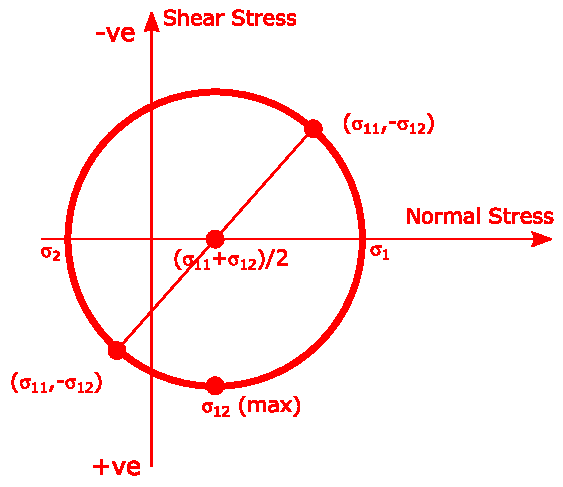
\includegraphics[height=7cm]{mohrs_circle_construction}
\end{figure}

\subsubsection{Examples of Mohr's circle}

(a) Uniaxial Tension, $\sigma_{11} = \sigma_{1}$

\begin{annotation}
$\sigma_{ij} = \begin{bmatrix}
\sigma_1 & 0 & 0 \\
0 & 0 & 0 \\
0 & 0 & 0
\end{bmatrix}$  \qquad 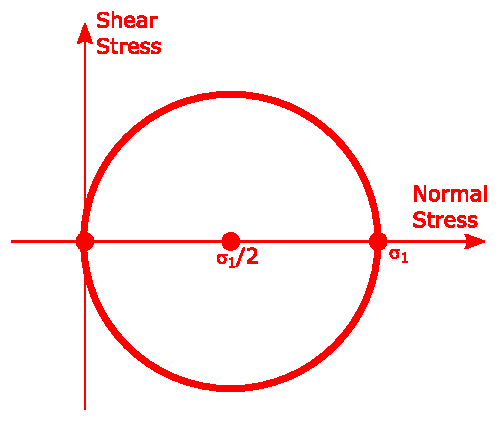
\includegraphics[width=6cm]{mohrs_uniaxial_tension}
\end{annotation}
\\

(b) Biaxial stress with equal compression and tension, $\sigma_{11} = \sigma_1, \sigma_{22}=-\sigma_1$

\begin{annotation}
$\sigma_{ij} = \begin{bmatrix}
\sigma_1 & 0 & 0 \\
0 & -\sigma_1 & 0 \\
0 & 0 & 0
\end{bmatrix}$  \qquad 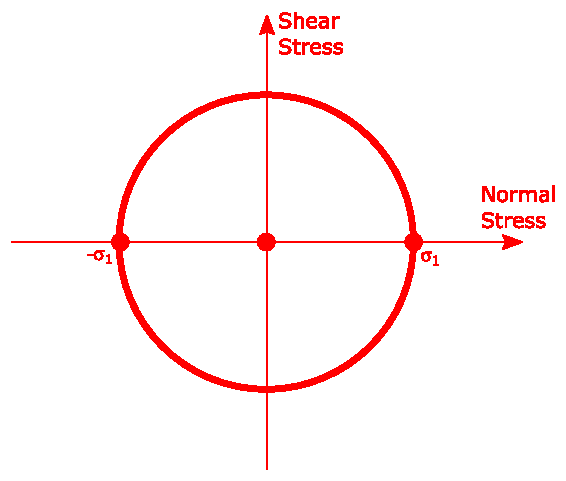
\includegraphics[width=6cm]{mohrs_biaxial_tension_compression}
\end{annotation}
\\
\begin{annotation}


We can represent the rotation of the frame of reference about each of the three principal axes:\\
{\hspace{4cm}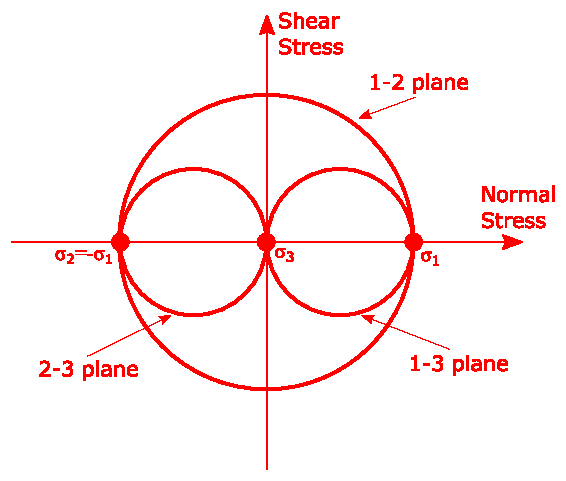
\includegraphics[width=6cm]{mohrs_biaxial_tension_compression_complete}}
\end{annotation}

(c) Triaxial Tension, $\sigma_{11}=\sigma_1, \sigma_{22}=\sigma_2, \sigma_{33}=\sigma_3$ (convention is that $\sigma_1>\sigma_2>\sigma_3$


\begin{annotation}
$\sigma_{ij} = \begin{bmatrix}
\sigma_1 & 0 & 0 \\
0 & \sigma_2 & 0 \\
0 & 0 & \sigma_3
\end{bmatrix}$  \qquad 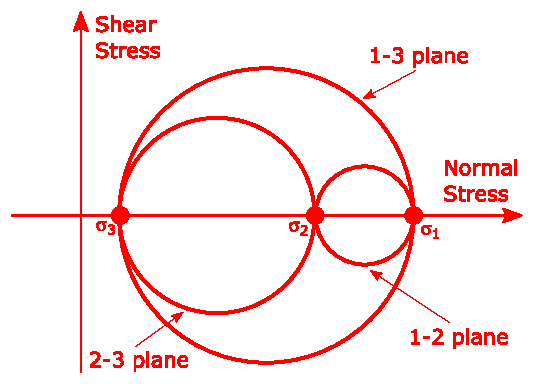
\includegraphics[width=6cm]{mohrs_triaxial_tension}
\end{annotation}
\\


% Example use of Mohr's circle here?

\subsection{Strain - a full treatment}

We have thus far dealt with stresses that arise due to applied forces on a material. These stresses cause deformations in a material, either reversible (elastic) or irreversible (plastic). We will first address the reversible strains, which tend to be limited to somewhat less than \SI{1}{\percent} (except in extreme cases like rubbery polymers).

Much like the stress tensor, the strain tensor must also be symmetrical. For stresses this removed the effect of net moments on a body, in the case of strains this is removing any rigid body rotation that is not associated with any deformation in the material itself. This is relevant to the simple deformation of shear strain given at the beginning of the course, which we will see includes a component of rotation.

\subsubsection{Relative displacement tensor}

Considering before and after a stress state is induced by  appling forces to a material, there will be resultant set of displacements of all points away from their initial positions. Assuming that the material is homogeneous, the displacements will be related to the stress state by the elastic properties of the material.

The \emph{relative displacement tensor} or \emph{deformation tensor} is a second rank tensor that defines how any point is displaced from it's initial position including normal and shear components in all three real space dimensions.

The components of the relative displacement tensor are defined by:
\begin{equation}
e_{ij} = \frac{\partial u_i}{\partial x_j}
\end{equation}
where $u_i$ is the displacement in the $i$th axis and $x_j$ is the position along the reference $j$th axis. These are dimensionless ratios of two distances. This is shown for the 2-3 plane in \autoref{fig:displacement_tensor}.
\FloatBarrier

\begin{figure}[h!]
\centering
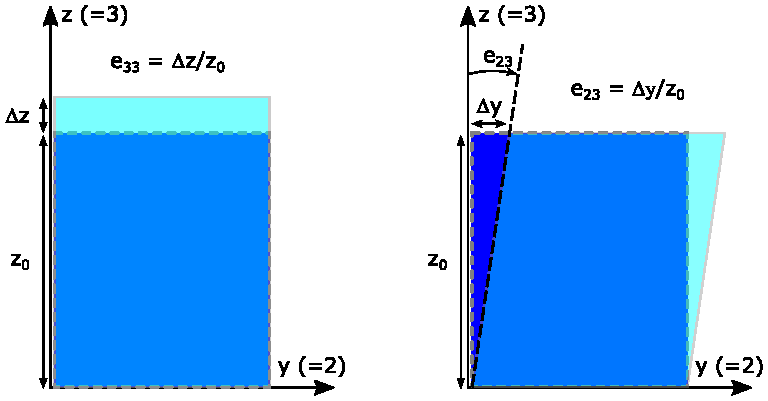
\includegraphics[width=0.8\textwidth]{displacement_tensor}
\caption{Illustration in the y-z (2-3) plane of how the relative displacement terms are defined. Note that $e_{23}$ (and other shear terms) can be considered angles when displacements are small. Conventionally the shear components are taken to be positive when the effect is to rotate the ositive reference axis towards the positive displacement axis, i.e. here rotating the positive 3-axis (reference) towards the positive 2-axis (displacement).\label{fig:displacement_tensor}}
\end{figure}

The definition of the shear term in \autoref{fig:displacement_tensor} is the same as the definition of simple shear given at the beginning of the course. However, this definition does not necessarily result in a symmetric tensor, in the situation shown in \autoref{fig:displacement_tensor} it is clear that $e_{23}\neq e_{32}$, since $e_{23}= \Delta y / z_0$ but $e_{32}=0$. Indeed, in general the displacement tensor is not constrained, and so is made up of two components, one symmetric component, strain, and one anti-symmetric component, rigid rotation, as shown in \autoref{fig:disp_strain_rotate}.


\FloatBarrier

\begin{figure}[h!]
\centering
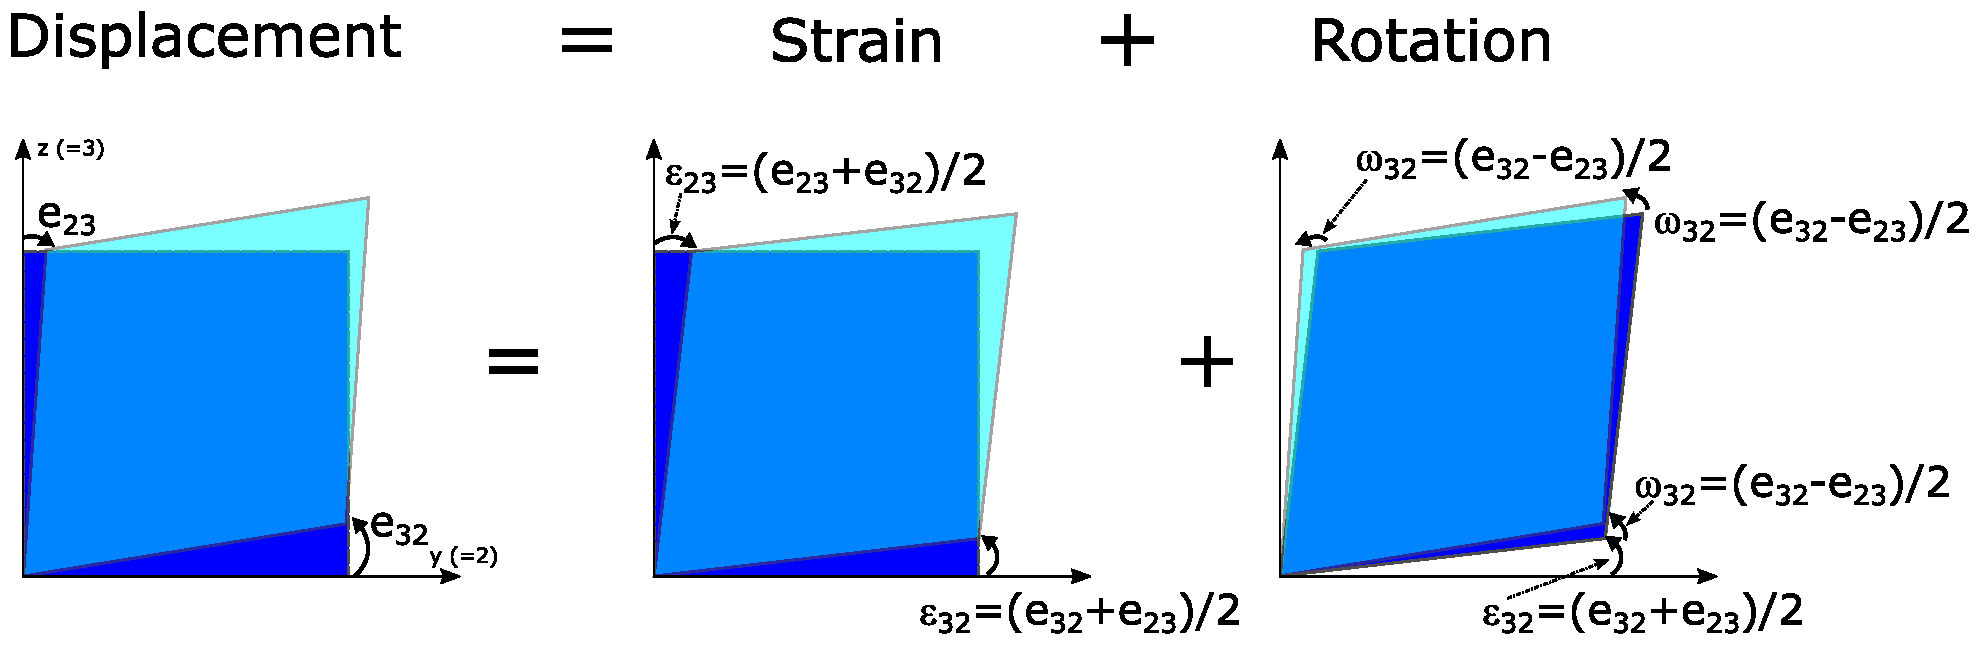
\includegraphics[width=\textwidth]{displacement_strain_rotation}
\caption{Schematic showing that a general displacements ($e_{23},e_{32}$) can be represented by  strains ($\varepsilon_{23} = \varepsilon_{32}$) and a rotation ($\omega_{23}=-\omega_{32}$).\label{fig:disp_strain_rotate}}
\end{figure}

\FloatBarrier

In general a second rank tensor can be expressed as a symmetric component and an antisymmetric component:\\
\begin{annotation}
\begin{equation}
e_{ij} = \dfrac{1}{2}(e_{ij} + e_{ji}) + \dfrac{1}{2}(e_{ij} - e_{ji}) \\
\end{equation}
\\
or for the specific case illustrated above:
\begin{equation}
e_{23} = \dfrac{1}{2}(e_{23} + e_{32}) + \dfrac{1}{2}(e_{23} - e_{32})
\end{equation}


Strain is the symmetric component: $\varepsilon_{ij}=\varepsilon_{ji}$\\
Rotation is the antisymmetric component: $\omega_{ij} = - \omega_{ji}$
\end{annotation}



 So the two components of a general displacement are:
\begin{align}
\text{Strain} \qquad \qquad & \qquad \qquad \text{Rotation} \nonumber \\
\varepsilon_{ij} = \dfrac{1}{2}(e_{ij} + e_{ji}) \qquad & \qquad \omega_{ij} = \dfrac{1}{2}(e_{ij} - e_{ji})
\end{align}

The definition of $\omega_{ij}$ means that itis antisymmetric and the leading diagonal is zero, and it easy to see that it represents a rigid body rotation, for example in 2D:
\begin{equation}
\omega_{ij} = \begin{bmatrix}
0 & \omega \\
-\omega & 0 
\end{bmatrix}
\end{equation}
results in a rotation:
\FloatBarrier
\begin{figure}[h!]
\centering
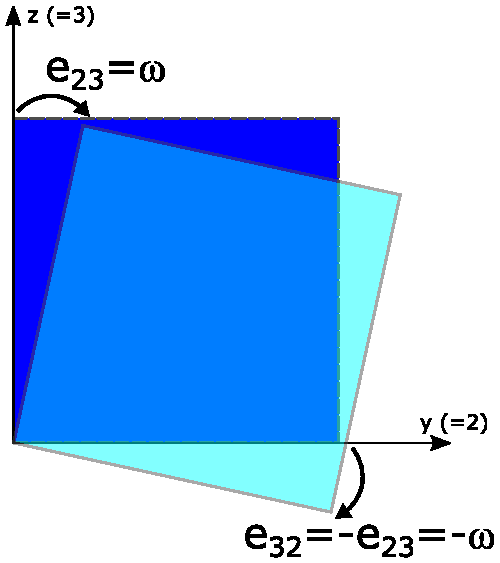
\includegraphics[width=0.5\textwidth]{rotation}
\caption{Schematic showing the rigid body rotation that arises from the anti-symmetric component of a general displacement tensor.}
\end{figure}
\FloatBarrier


Normally we do not consider the rigid body rotation further, it may be important from a structures point of view, but for the material itself it is not relevant.

Since strain is a second rank tensor, like the stress tensor it can be diagonalised to give the principal strains and like principal stresses, these are normal stresses that act in principal directions which experience no shear strain. The same matrix transformations apply and constructions like Mohr's circle can be used.

For completeness the full strain tensor is given by:
\begin{equation}
\begin{bmatrix}
\varepsilon_{11} & \varepsilon_{12} & \varepsilon_{13} \\
\varepsilon_{12} & \varepsilon_{22} & \varepsilon_{23} \\
\varepsilon_{13} & \varepsilon_{23} & \varepsilon_{33}
\end{bmatrix}
=
\begin{bmatrix}
e_{11} & ^1\!/_2 (e_{12} + e_{21}) & ^1\!/_2 (e_{13} + e_{31}) \\
^1\!/_2 (e_{21} + e_{12}) & e_{22} & ^1\!/_2 (e_{23} + e_{32}) \\
^1\!/_2 (e_{31} + e_{13}) & ^1\!/_2 (e_{32} + e_{23}) & e_{33}
\end{bmatrix}
\end{equation}
and when referred to principal axes this becomes:
\begin{equation}
\varepsilon_{ij} = \begin{bmatrix}
\varepsilon_1 & 0 & 0 \\
0 & \varepsilon_2 & 0 \\
0 & 0 & \varepsilon_3
\end{bmatrix}
\end{equation}


\subsubsection{Hydrostatic and deviatoric strains}

The strain tensor can be described as the sum of two components, a hydrostatic and deviatoric components. In broad terms the hydrostatic component is the strain associated with a change in volume and the deviatoric component is the strain associated with shape changes without any volume strain.

Considering an element of material subjected to principal strains $\varepsilon_1, \varepsilon_2$ and $\varepsilon_3$. The volumetric strain (see IA course E) can be written as:
\begin{equation}
\Delta = (1+\varepsilon_1)(1+\varepsilon_2)(1+\varepsilon_3) -1 = \varepsilon_1 + \varepsilon_2 + \varepsilon_3 + O(\varepsilon^2)
\end{equation}
The higher order terms can be ignored for small strains. This is equivalent to the trace of the tensor, and this is invariant under any transformation of reference axes, so this can be written succinctly in suffix notation:
\begin{equation}
\Delta = \varepsilon_{ii}
\end{equation}

The hydrostatic component of a general strain will therefore have the form:
\begin{equation}
\varepsilon_{ij} = \begin{bmatrix}
^{\Delta}\!/_3 & 0 & 0 \\
0 & ^{\Delta}\!/_3 & 0 \\
0 & 0 & ^{\Delta}\!/_3
\end{bmatrix}
\end{equation}
and the other component follows:
\begin{equation}
\begin{bmatrix}
\varepsilon_{11} & \varepsilon_{12} & \varepsilon_{13} \\
\varepsilon_{12} & \varepsilon_{22} & \varepsilon_{23} \\
\varepsilon_{13} & \varepsilon_{23} & \varepsilon_{33}
\end{bmatrix}
= \begin{bmatrix}
\Delta/3 & 0 & 0 \\
0 & \Delta3 & 0 \\
0 & 0 & \Delta/3
\end{bmatrix}
+ \begin{bmatrix}
\varepsilon_{11} - ^{\Delta}\!/_3 & \varepsilon_{12} & \varepsilon_{13} \\
\varepsilon_{12} & \varepsilon_{22} - ^{\Delta}\!/_3 & \varepsilon_{23} \\
\varepsilon_{13} & \varepsilon_{23} & \varepsilon_{33} - ^{\Delta}\!/_3
\end{bmatrix}
\end{equation}

\begin{annotation}
\qquad\qquad General strain \qquad\quad hydrostatic \qquad\qquad\qquad\qquad deviatoric
\end{annotation}

The effects of these individual components are shown schematically in \autoref{fig:strain_components}.
\begin{figure}
\centering
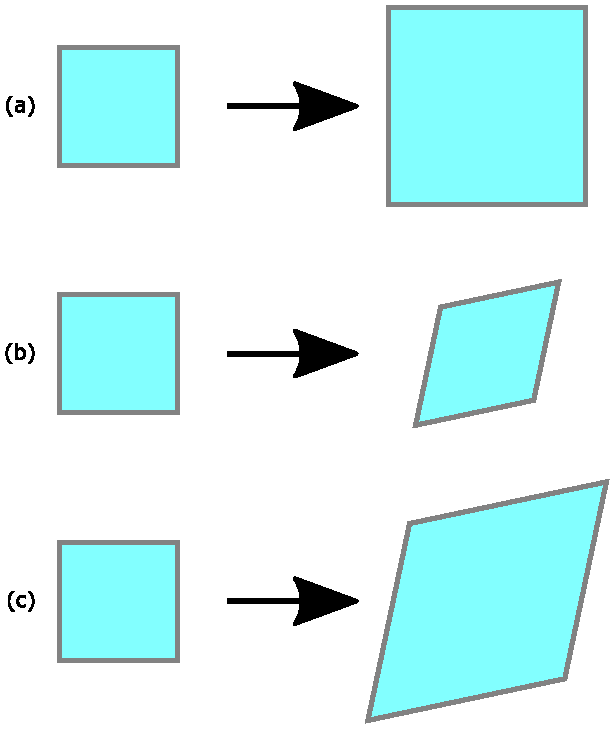
\includegraphics[width=0.5\textwidth]{strain_components}
\caption{Schematic showing the effects of (a) a hydrostatic strain, (b) a deviatoric strain and (c) a general strain made up of both components.\label{fig:strain_components}}
\end{figure}


\subsubsection{Shear strain - engineering vs tensor definitions}

There is a minor complication in our descriptions of shear strains. Our tensor definition includes shear terms, for example $\varepsilon_{12}$, so it might be expected that the shear modulus would be defined by the ratio of $\varepsilon_{12}/\sigma_{12}$. Unfortunately $G\neq \varepsilon_{12}/\sigma_{12}$. The problem is to do with our original definition of the shear modulus, see \autoref{eqn:def_moduli}. We might write this with suffices as:
\begin{equation}
G=\frac{\sigma_{12}}{\gamma_{12}} \qquad \qquad \qquad \begin{annotation}
G = \frac{\tau}{\gamma}
\end{annotation}
\end{equation}
where $\gamma_{12}$ is the simple strain, with  no account made for the fact that this should be represented as two shear strains ($\varepsilon_{12}=\varepsilon_{21}$) and a rigid body rotation ($\omega_{12}=-\omega_{21}$). This is shown in \autoref{fig:tensor_vs_engineer_shear}.
\FloatBarrier
\begin{figure}
\centering
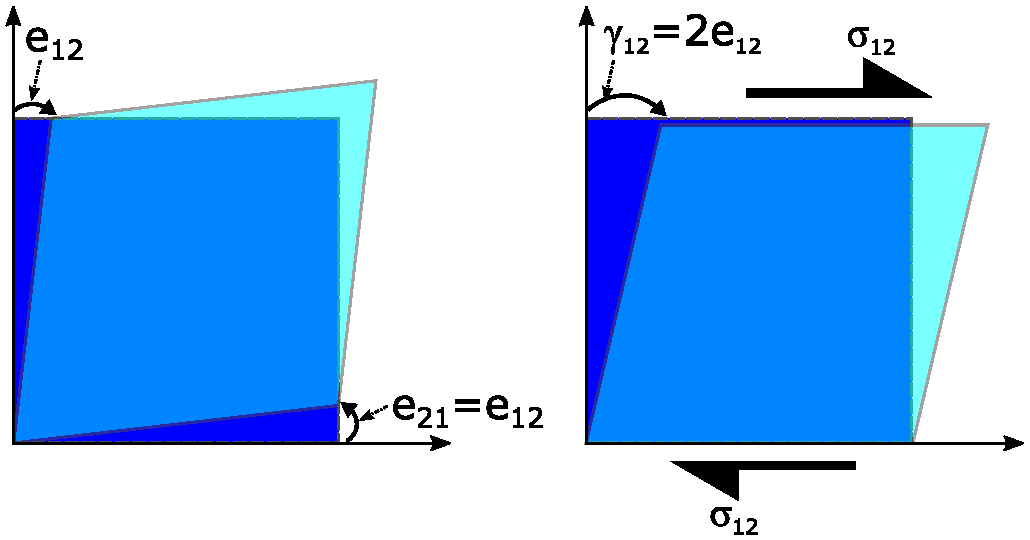
\includegraphics[width=0.6\textwidth]{tensor_vs_engineering_shear}
\caption{Schematic showing the difference between tensor shear (left) where two components describe the shape change, and there is no rotation, and engineering shear, right, where a single component describes the shear and includes an implicit rotation.\label{fig:tensor_vs_engineer_shear}}
\end{figure}
\FloatBarrier
This means that the shear modulus is instead defined by the equation:
\begin{equation}
G=\frac{\sigma_{12}}{\gamma_{12}}
\end{equation}
and that the engineering strains, $\varepsilon_{ii}$ and $\gamma_{ij}$, do not form a tensor and therefore can't be manipulated using tensor methods discussed here, such as axis transformation or relation to stress via the stiffness or compliance tensor. That said, the simple shear modulus can be related to the tensor formulation:

\begin{align}
\varepsilon_{12} = S_{1212}\sigma_{12} + S_{1221}\sigma_{21} = 2 S_{1212}\sigma_{12}\nonumber \\
 G = \frac{\sigma_{12}}{\gamma_{12}} = \frac{\sigma_{12}}{2\varepsilon_{12}} = \frac{1}{4S_{1212}}
\end{align}

For isotropic materials this sort of analysis can be done to link simple elastic engineering constants (Young's modulus, bulk modulus, shear modulus, Poisson ratio etc.) with the components of the compliance and stiffness tensors. In fact there are only two independent constants so $E$ and $\nu$ are sufficient. Where materials are anisotropic there are more independent components and the analysis becomes more difficult.



\subsection{Stiffness and Compliance}

We are used to the idea that in a simple uniaxial stress state the strain is linked to stress by the equation:
\begin{equation}
\sigma = E \varepsilon
\end{equation}
when using stress and strain tensors for general cases this relationship becomes:
\begin{equation}
\sigma_{ij} = C_{ijkl}\varepsilon_{kl} \label{eqn:hookes_law}
\end{equation}
where $C_{ijkl}$ is called the stiffness tensor. Since both stress and strain are second rank tensors, and all the components of strain could have a dependence on all the components of stress the stiffness is a fourth rank tensor (in general a tensor that relates an $n$th rank and an $m$th rank tensor will have a rank of $n+m$). The stiffness will therefore have $3\times3\times3\times3$ components (81!).  

\autoref{eqn:hookes_law} is the generalised form of Hooke's law, and materials that obey this are said to be \emph{linearly elastic}. The inverse relationship can be written:
\begin{equation}
\varepsilon_{ij} = S_{ijkl} \sigma_{kl}
\end{equation}
where $S_{ijkl}$ is the compliance tensor. (Note the annoying convention that the letters representing stiffness and compliance are the reverse of the initial letter of each word.)

\subsubsection{Constraints on the stiffness tensor}

In principal there are a large number of terms to deal with for a general stress state and this is tedious if not daunting, however there are various constraints that limit the number of terms that need to be considered in most cases.

One constraint that always applies is that the body is in static equilibrium, and as a result the stress and strain tensors are symmetrical, such that $\sigma_{ij}=\sigma_{ji}$ and $\varepsilon_{kl}=\varepsilon_{lk}$. Thus the $i$ and $j$ indices can be swapped without effect, and similarly $k$ and $l$. This means that:
\begin{equation}
C_{ijkl}=C_{jikl}=C_{ijlk}=C_{jilk}
\end{equation}
This reduces the components from 81 to 36. Furthermore there is usually some symmetry inherent to the material that reduces this number further, for example the response of a cubic material to an applied stress will not vary under a transformation that maps [1\,0\,0] to the [0\,1\,0]. For a cubic material there are only three independent elastic constants. For a completely isotropic material, like glass or a randomly oriented polycrystal there re only 2 independent elastic constants.

\subsubsection{Relationship to Young's modulus}

It is tempting to relate the tensor stiffness to elastic constants by considering  the application of one normal stress and a single normal strain arising as a result:
\begin{equation}
\sigma_{11} = E \varepsilon_{11}
\end{equation}
where $E$ is the Young's modulus which we are familiar with. From this one might conclude that $C_{1111}=E$. This is not correct though, because the application of a single stress does not give rise to a single strain due to Poisson strains:
\FloatBarrier
\begin{figure}[h!]
\centering
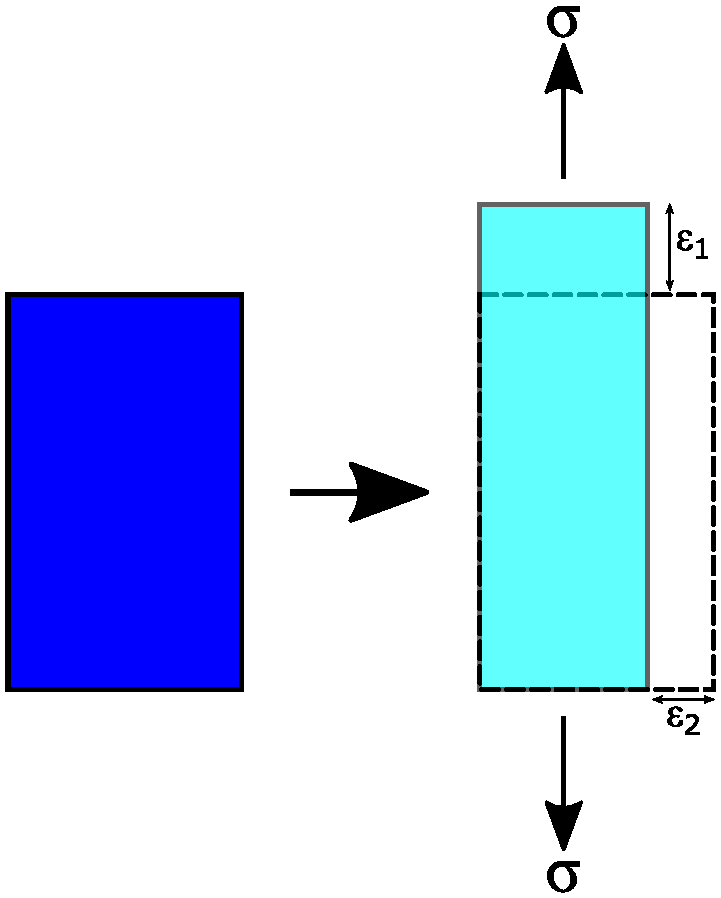
\includegraphics[width=4cm]{poisson_strains}
\end{figure}
\FloatBarrier

This means that there are in fact three strain terms that depend on the single stress in the full tensor description of the situation. However, if we instead consider this in terms of compliance then Young's modulus can be related to the tensor elastic constants:
\begin{equation}
\varepsilon_{11} = S_{1111}\sigma_{11}
\end{equation}
Now there is only one stress term and ne strain term relevant to the equation and therefore Young's modulus is:
\begin{equation}
E = \frac{1}{S_{1111}}
\end{equation}

\subsubsection{Relationship to the Poisson ration}

The Poisson ratio, represented by the symbol $\nu$, gives the transverse contraction that arises as a result of a axial tensile strain. Considering the application of a single normal stress, $\sigma_{1}$ generating principal strains $\varepsilon_1, \varepsilon_2$ and $\varepsilon_3$, the Poisson ratio is defined to be:
\begin{equation}
\varepsilon_2 = -\nu \varepsilon_1 \label{eqn:poisson_definition}
\end{equation}
and in tensor notation we can write:
\begin{equation}
\epsilon_2 = S_{2211}\sigma_1 \begin{annotation}
= S_{1122}\sigma_1
\end{annotation}
\end{equation}

Using the definition of Young's modulus we can substitute for $\varepsilon_1$ in \autoref{eqn:poisson_definition}:
\begin{equation}
\varepsilon_2 = -\nu \frac{\sigma_1}{E}
\end{equation}
and substituting for $\varepsilon_2$:
\begin{equation}
S_{1122} \sigma_1 = -\frac{\nu}{E} \sigma_1
\end{equation}
so
\begin{equation}
S_{1122} = -\frac{\nu}{E}
\end{equation}

During multiaxial loading (i.e.\ with more than one non-zero principal stress) the Poisson strains superimpose this leads to a set of equations for the principal strains that arise from an applied set of principal stresses (for an isotropic material):
\begin{align}
\varepsilon_1 = \frac{\sigma_1}{E} - \nu \frac{(\sigma_2 + \sigma_3)}{E} \nonumber\\
\varepsilon_2 = \frac{\sigma_2}{E} - \nu \frac{(\sigma_1 + \sigma_3)}{E}  \label{eqn:constitutive_laws}\\
\varepsilon_3 = \frac{\sigma_3}{E} - \nu \frac{(\sigma_1 + \sigma_2)}{E} \nonumber 
\end{align}


































































\clearpage

\section{Mechanics of structures}

The aim of this section is not to give a comprehensive grounding in structures, there are structural engineers for that sort of thing, but to at least look at the basics to see how material choices and structural design choices can be linked.

\subsection{Recap of bending moments and beam stiffness}

A moment, $M$, is generated by the application of a force (or forces) with some transverse separation. It is calculated by:
\begin{equation}
M = FL
\end{equation}
where $F$ is the component of the forces perpendicular to the separation $L$. Using this we can calculate how a moment varies along a cantilever loaded at one end and fixed at the other:

\FloatBarrier
\begin{figure}[h!]
\centering
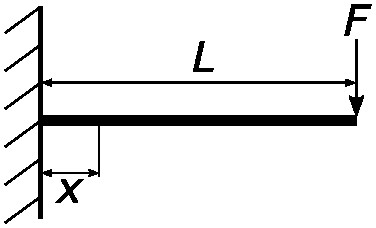
\includegraphics[width=0.5\textwidth]{end_loaded_cantilever}
\caption{A cantilever fixed at one end and loaded transversely at the other.\label{fig:simple_cantilever}}
\end{figure}
\FloatBarrier

This gives a moment at a position $x$ of:
\begin{equation}
\begin{annotation}
M=F(L-x)
\end{annotation}
\end{equation}
And this can be extended to multiple forces:
\FloatBarrier
\begin{figure}
\centering
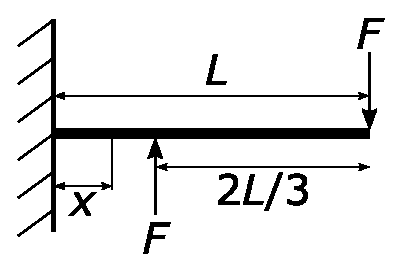
\includegraphics[width=0.5\textwidth]{two_forces_cantilever}
\caption{A cantilever with two applied forces.}
\end{figure}
\FloatBarrier
This gives the moment at the point $x$ as:
\begin{equation}
\begin{annotation}
M=F(L-x) - F(L/3 - x)
\end{annotation}
\end{equation}

This is then linked to the material by the beam stiffness equation:
\begin{equation}
M=\kappa EI \label{eqn:beam_bending}
\end{equation}
where $I$ is the second moment of area and is calculated by:
\begin{equation}
 I = \int_A y^2 dA 
\end{equation}
where $dA$ is an element of area at a distance $y$ from the neutral axis.

This can be applied even to complex arrangements of forces along beams or even distributed forces, as long as an expression for the moment at any point is obtainable.

We can find the deflection of a point along the beam by approximating the second derivative of the height of the beam as equal to the curvature:
\FloatBarrier
\begin{figure}[h!]
\centering
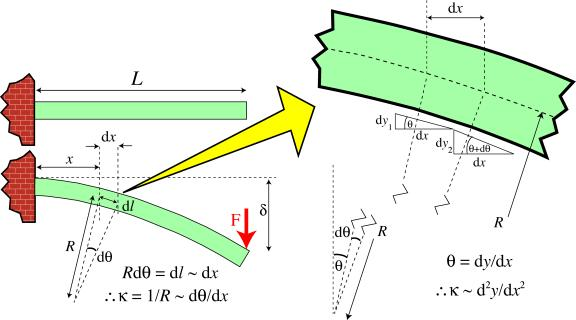
\includegraphics[width=\textwidth]{moment_diagram1}
\caption{The approximation, valid for small deflections, that the curvature of the beam and of the neutral axis are equal. Reproduced from \cite{doitpoms_beams}.}
\end{figure}
\FloatBarrier

This gives us:
\begin{equation}
\kappa = \frac{d^2y}{dx^2}
\end{equation}

and we can substitute this into the beam bending equation (\autoref{eqn:beam_bending}):
\begin{equation}
\frac{d^2y}{dx^2}=\kappa = \frac{M}{EI} \label{eqn:beam_curvature}
\end{equation}

Using this we can use the balance of moments between the internal moments and external moments to find an expression for the shape of the deformed beam.

Considering the end loaded cantilever above we can write:
\begin{equation}
EI \frac{d^2y}{dx^2} = M = F(L-x)
\end{equation}
where $x$ is as defined in \autoref{fig:simple_cantilever}. This can be integrated:
\begin{equation}
EI\frac{dy}{dx} = FLx - \frac{Fx^2}{2} + c_1
\end{equation}
Since at the wall, $x=0$ and $\frac{dy}{dx} = 0$, the constant $C_1=0$. We can then integrate again:
\begin{equation}
EIy = \frac{FLx^2}{2} - \frac{Fx^3}{6} + C_2
\end{equation}
Again, the boundary condition that at $x=0$, $y=0$ so therefore $C_2=0$, giving the final expression:
\begin{equation}
y = \frac{Fx^2}{6EI}(3L-x)
\end{equation}
and therefore the maximum deflection is
\begin{equation}
\delta = \frac{FL^3}{3EI} \qquad \begin{annotation}\text{and this occurs at} \,\, x=L
\end{annotation}
\end{equation}


Problems of this type are all solved in this manner, balancing the moments de to the internal stresses and an externally applied moment. There are two main challenges, the first is to find an expression for the external moment, which can be complex if there is more than one force applied. This expression can and will vary along the length of the beam, changing as the reference point passes the position of applied forces.

The second key point is to identify the boundary conditions, which usually rely on known fixed points where the displacement, or the gradient must be zero, or that the beams displacement and gradient must be continuous.









\subsubsection{The parallel axis theorem}


This can be adjusted to be about another parallel axis displaced by a distance $d$ form the neutral axis:
\begin{equation}
I_{\text{parallel}} = \int_A (y+d)^2dA = \int y^2 dA + 2 d \int y dA + d^2\int dA
\end{equation}

Since the distance $y$ is to the neutral axis, the second term must be zero (the neutral axis passes through the centre of mass). This leaves what is know as the parallel axis theorem:
\begin{equation}
I_{\text{parallel}} = I_{\text{neutral}} + d^2A
\end{equation}

\subsubsection{Stresses and strains in a beam}

To recap from IA, the strains in a bent beam can be found straight forwardly from the diagram in \autoref{fig:strain_from_curvature}.
\FloatBarrier
\begin{figure}[h!]
\centering
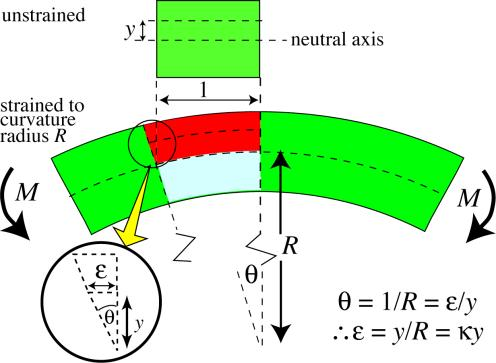
\includegraphics[width=0.5\textwidth]{bend_diagram2}
\caption{The relationship between curvature and strain in a bent beam. Reproduced from the DoITPoMS TLP \cite{doitpoms_beams}.\label{fig:strain_from_curvature}}
\end{figure}
\FloatBarrier

If we assume that the deformation remains elastic then we can relate the strain to the stress simply by: $\sigma = E \varepsilon = E\kappa y$

This can be used to derive the beam bending equation:

\FloatBarrier
\begin{figure}[h!]
\centering
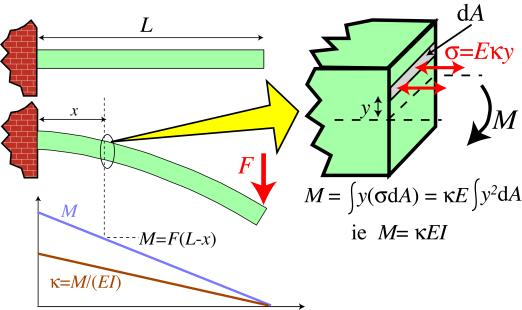
\includegraphics[width=0.8\textwidth]{bend_diagram}
\caption{The balance between the externally applied moments and the internally generated moments due to stresses.\label{}}
\end{figure}
\FloatBarrier

\subsubsection{Torsion}

Torsion is the application of a {\bf torque (twisting moment)} to induce a {\bf twist} in a beam. Torques are common in engineering situations, for example in service for shafts in engines and bridges, but also in construction in screws and bolts. They can also arise is more unexpected places such as boat hulls or aeroplane fuselages. 

A torque (usually denoted $T$) has the same units (\si{\newton\meter}) as bending moments (usually $M$), as both are a product of a force and a perpendicular distance. The difference is in their orientation relative to the beam. Bending moments are parallel to the radius (of a round beam), and act through the beam; a torque is a tangential force that is offset radially from the axis of rotation.

Torsion is simple for thin walled cylinders where the stress cannot vary much across the thickness of the wall, the problem becomes one of simple force balance:


\FloatBarrier
\begin{figure}[h!]
\centering
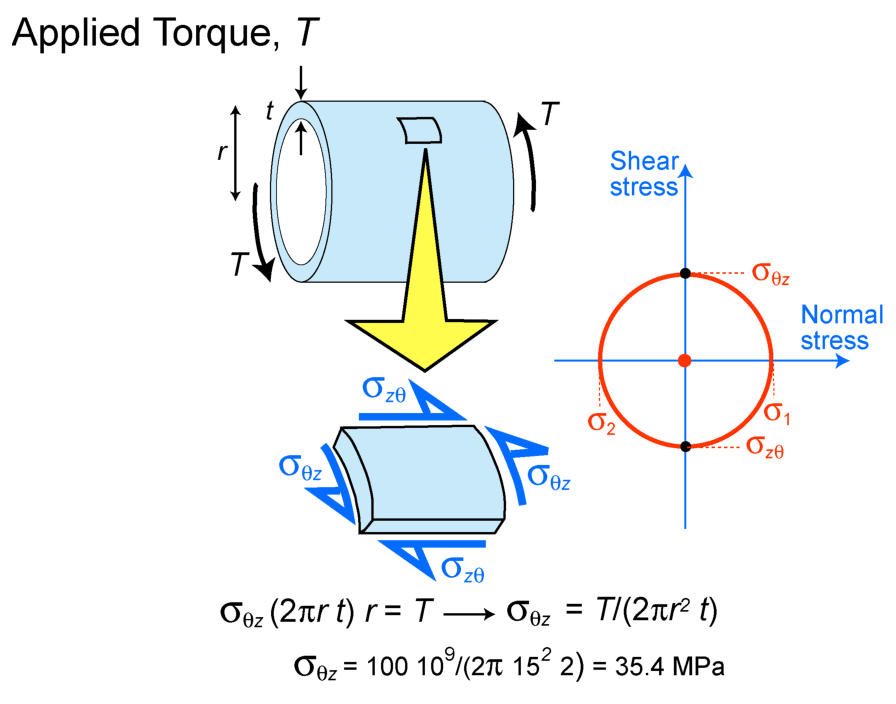
\includegraphics[width=0.6\textwidth]{thin_wall_torsion}
\caption{Stresses that arise due to a torsion applied to a thin walled cylinder. Mohr's Circle can be used to find the principal stesses.}
\end{figure}
\FloatBarrier
The result is:
\begin{align}
T= \sigma_{\theta z} (2\pi r t) r \nonumber \\
\implies \sigma_{\theta z} = \frac{T}{2 \pi r^2 t}
\end{align}


It is important to remember the assumptions that have been made in reaching this point (in fact it's always important). In this case the assumption relies on the wall being thin and therefore that the stresses do not vary significantly across the thickness of the wall. This is not the case for a solid cylindrical shaft or thick walled cylinders.

Since solid cylinders are more usual for transferring torque (e.g.\ drive shafts). In this case the stress will vary with the radial position.

\FloatBarrier
\begin{figure}[h!]
\centering
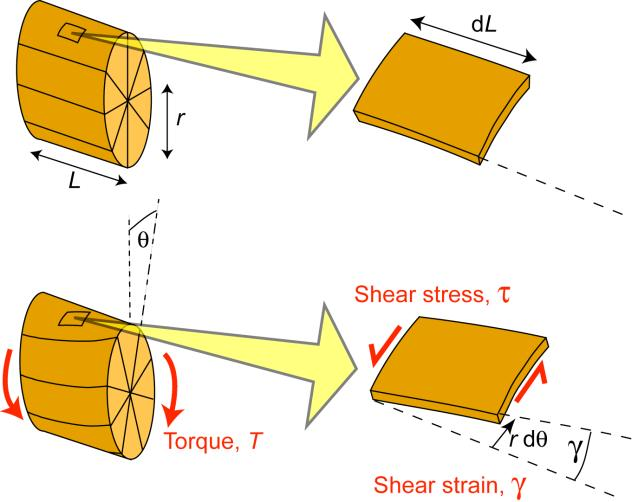
\includegraphics[width=0.55\textwidth]{twist_diagram}
\caption{The application of a torque to a solid cylinder and the development of shear strains.}
\end{figure}
\FloatBarrier


By considering a straight reference line along the axis of the shaft being displaced we can define the strain:

\FloatBarrier
\begin{figure}[h!]
\centering
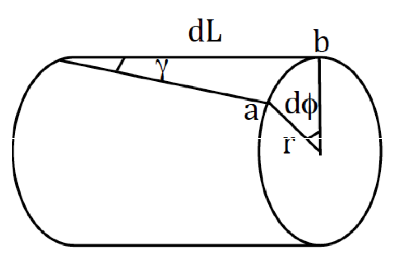
\includegraphics[width=0.3\textwidth]{torsional_strain}
\end{figure}
\FloatBarrier

The strain (the $\theta z$ component) is given by:
\begin{equation}
\begin{annotation}
\gamma_{\theta z} = d\frac{d\phi}{dL}
\end{annotation}
\end{equation}

Which we can relate to the overall twist in the bar to find the maximum shear strain (which will occur at the outside of the bar):
\begin{equation}
\gamma_{\theta z}^{\text{max}} = \frac{R\phi}{L}
\end{equation}
Assuming that the rate of twist can be calculated from the total angle of twist, $\phi$, and the total length of bar, $L$.

This can be converted to a stress by assuming that Hooke's Law holds (i.e.\ $\sigma_{\theta z} = G \gamma_{\theta z}$):
\begin{equation}
\sigma_{\theta z} = G r \frac{d\phi}{dL}
\end{equation}


We now have a handle on the force balance that must arise in equilibrium, i.e.\ the internal stresses must balance the external torque:

\begin{equation}
T = \int dT = \int \sigma_{\theta z} r dA = \int Gr^2 \frac{d\phi}{dL}dA
\end{equation}

By analogy with beam bending there is a geometric term which is the {\bf polar} second moment of area:
\begin{equation}
I_{\text{P}} = \int r^2 dA
\end{equation}
and there is also an expression equivalent to the beam bending equation ($M=EI\kappa$):
\begin{equation}
T = G I_{\text{P}} \frac{d\phi}{dL}
\end{equation}
where the rate of twist is the equivalent to the curvature of a cantilever.

%% NB a question on this might be to find the maximum stress for the drive shaft of a car engine (maybe even consider the weight/cost)
























































\clearpage

 \section{Plasticity and mechanical testing}
 
 \subsection{Dislocations}
  \FloatBarrier
In the IA course the behaviour of dislocations was covered in quite some detail, so this section will review and extend this.
 
To recap briefly, dislocations are linear defects that exist in crystalline materials and allow plastic deformation to occur. They are always of a slip system, which are defined by a slip direction, the relative displacement of atoms that result from their passage, and a slip plane, in which the dislocations move and across which the displacement happens, the displacement is the Burgers vector.
 
There are types of dislocations defined by the relative orientation of their line vector and Burgers vector, edge dislocations have their Burgers vector perpendicular to their line vector, while for screw dislocations these are parallel. For the purposes of this course we will mostly consider edge dislocations, though most of the analysis can be adapted to apply to screw dislocations.
 
In IA course E, the motion of dislocations was introduced as the mechanism that controls the strength of crystalline materials. The lower bound on strength was the lattice resistance or Peierls-Nabarro stress. Additionally, a number of strengthening mechanisms were introduced including:
\begin{itemize}
\item forest hardening
\item grain boundary hardening
\item solid solution strengthening
\item precipitate strengthening
order hardening
\end{itemize}

\begin{figure}[h!]
\centering
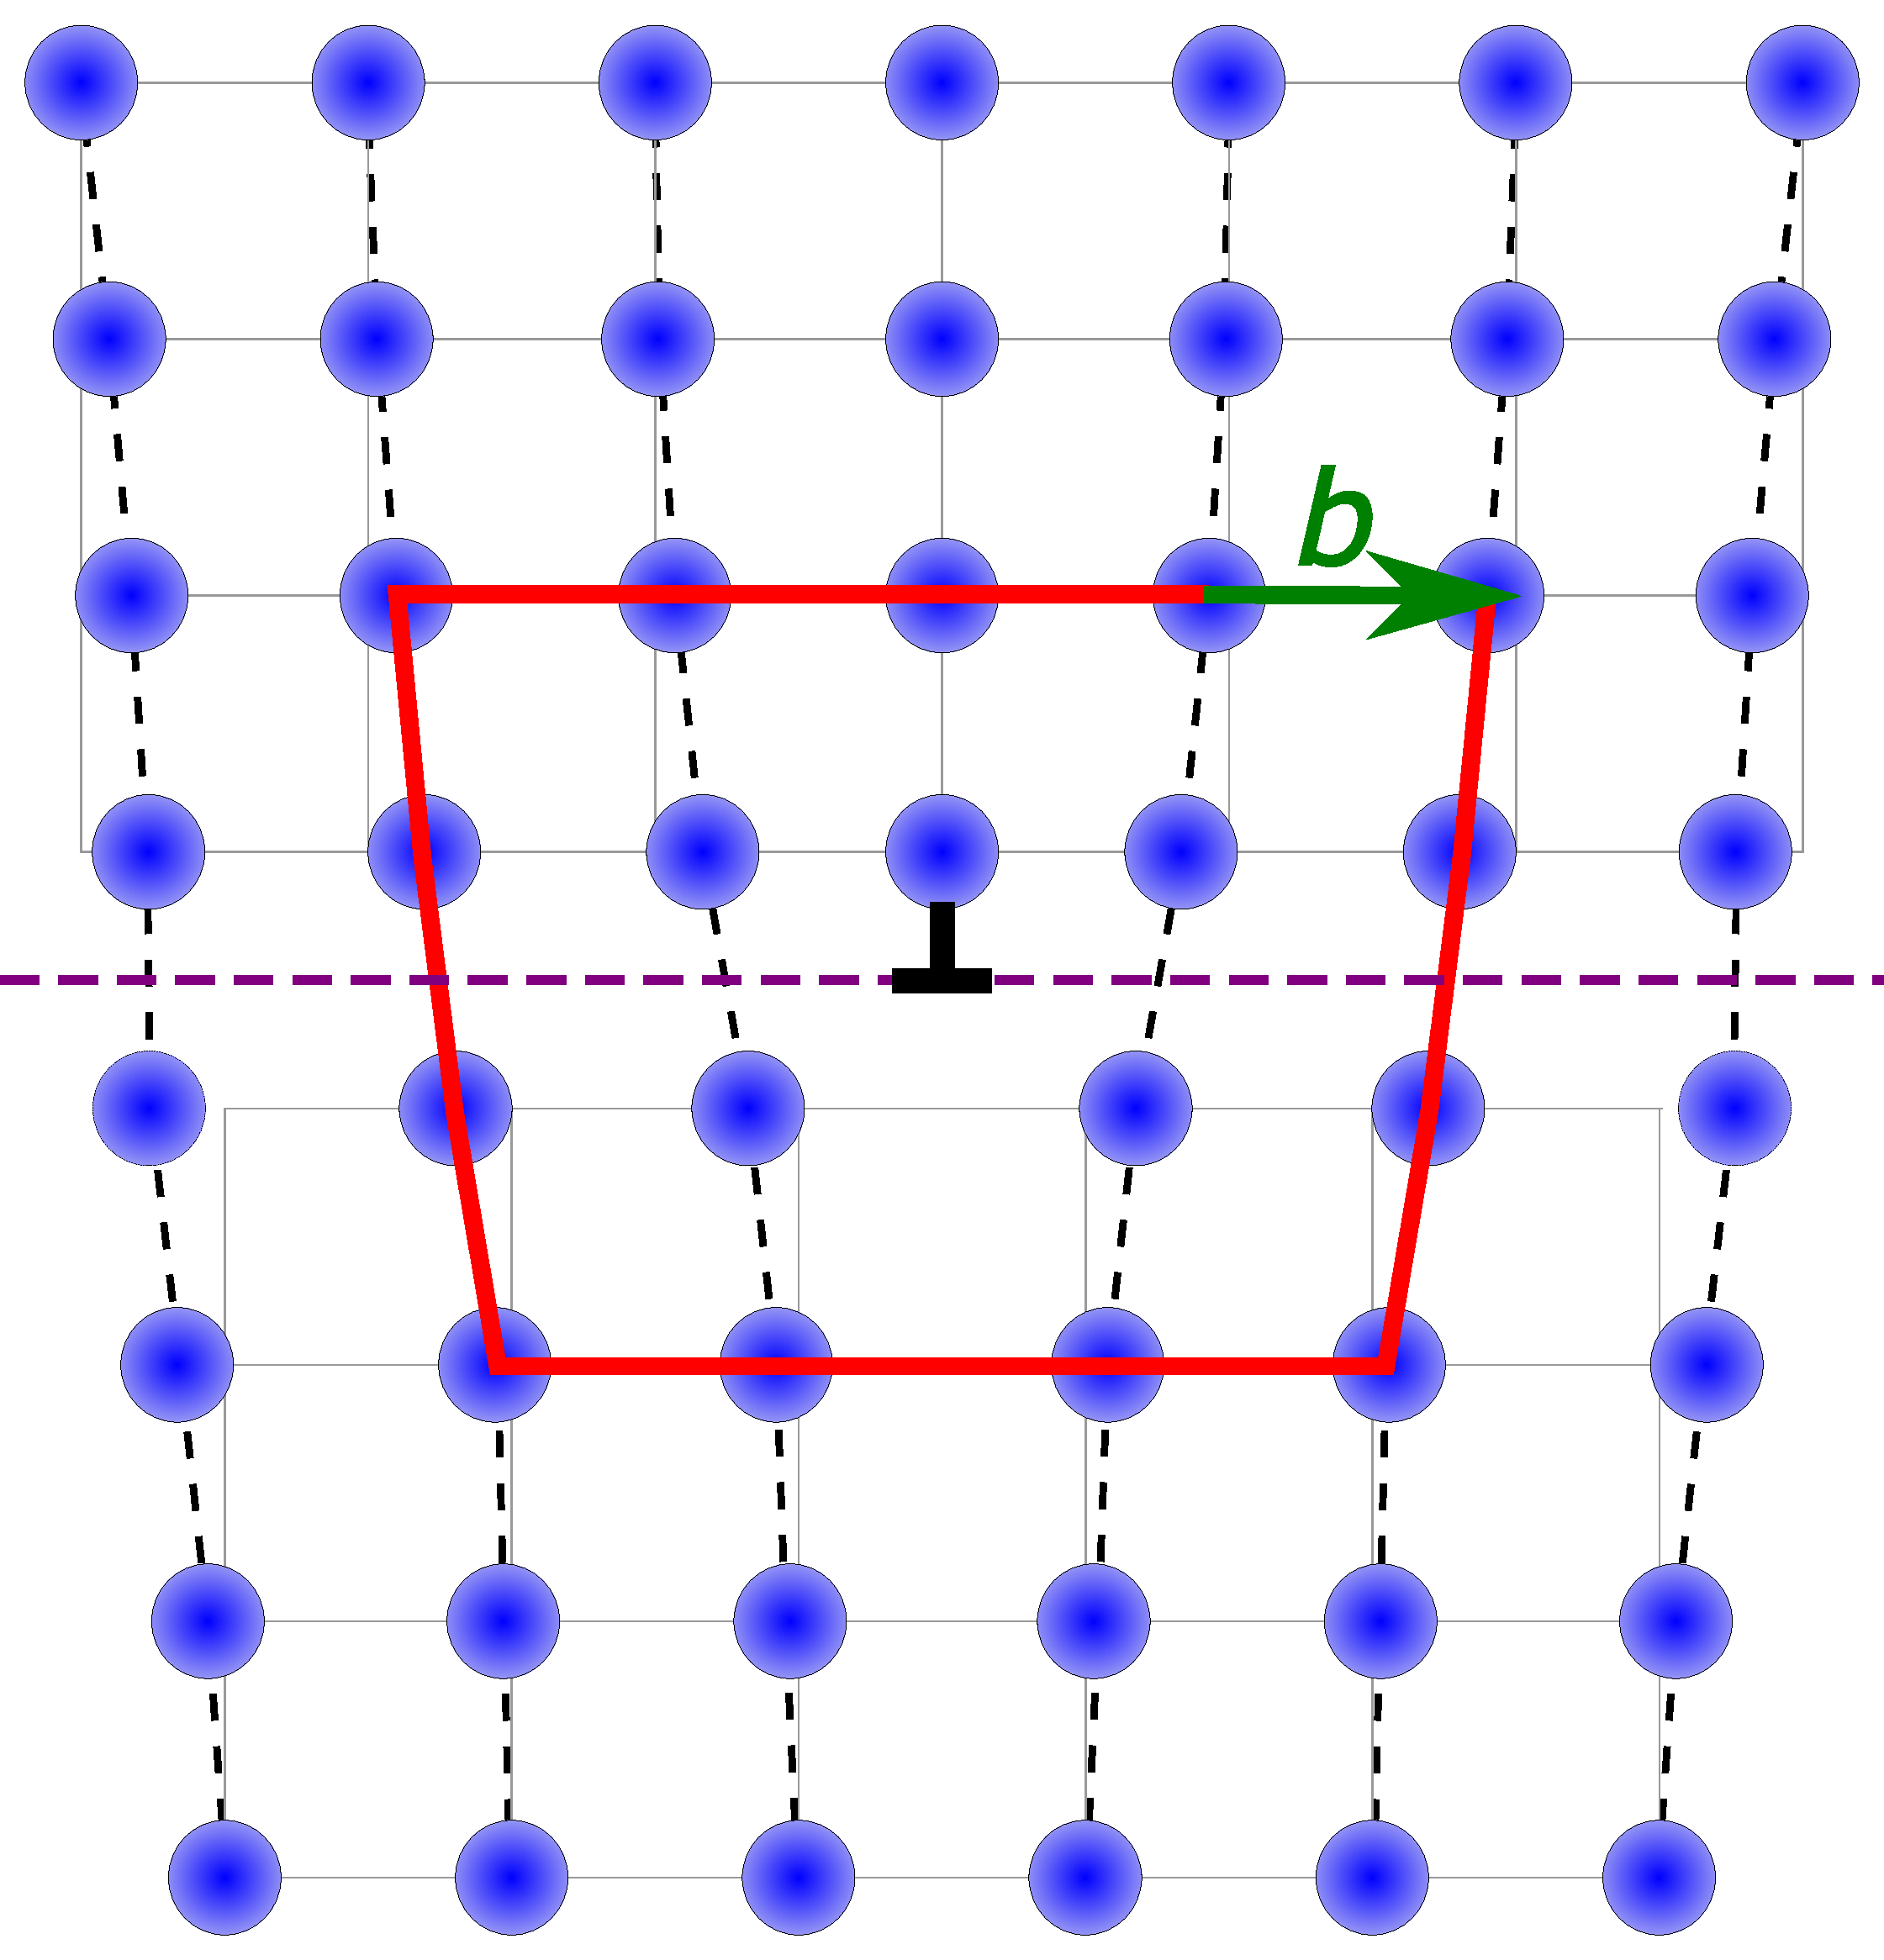
\includegraphics[width=0.6\textwidth]{Edge_Dislocation}
\caption{A schematic showing an edge dislocation, with the loop determined by a Burgers circuit. The slip plane is highlighted by the horizontal dashed line.}
\end{figure}
 
 
Here we will take a more in depth look at the lattice resistance and the way that work hardening occurs through the development of a dislocation network, introduced in IA as forest hardening.
\FloatBarrier

\subsubsection{The lattice resistance}

Dislocations were first considered as discontinuities in elastic continua, such a dislocation is called a ``Volterra'' dislocation. They are one of the classic problems of traditional continuum linear elasticity, however they cannot predict the behaviour of defects in a crystal which exist in a lattice.

It is precisely the periodicity of the crystal lattice that gives rise to a critical stress required to move a dislocation. The energy of a dislocation is not fixed, but will change as the dislocation moves with the same periodicity as the crystal lattice.

The energy changes associated with moving a dislocation were first examined mathematically by Rudolf Peierls and extended by Frank Nabarro. Their models have a common first step in examining the energy changes, which is to first calculate the energy of a dislocation.

\subsubsection*{Building a dislocation}
A dislocation can be created in a thought experiment by starting with two misaligned half crystals which are brought together at what becomes the slip plane.

The unit cells that span the slip plane will be experiencing large strains that will have a large associated energy. If we assume that the displacements normal to the slip plane are negligible, then there are two main components to the energy of either defects shown in \autoref{fig:making_a_disloc}: firstly there is a misalignment, essentially a shear strain across the slip plane with atoms displaced parallel to the slip with respect to the equilibrium neighbour across the slip plane. Secondly there will be a normal strain parallel to the slip plane, i.e.\ where the displacement parallel to the slip plane has brought neighbours {\bf in the same plane} too close together or too far apart.


\FloatBarrier
\begin{figure}[h!]
\centering
\begin{subfigure}{0.35\textwidth}
\centering
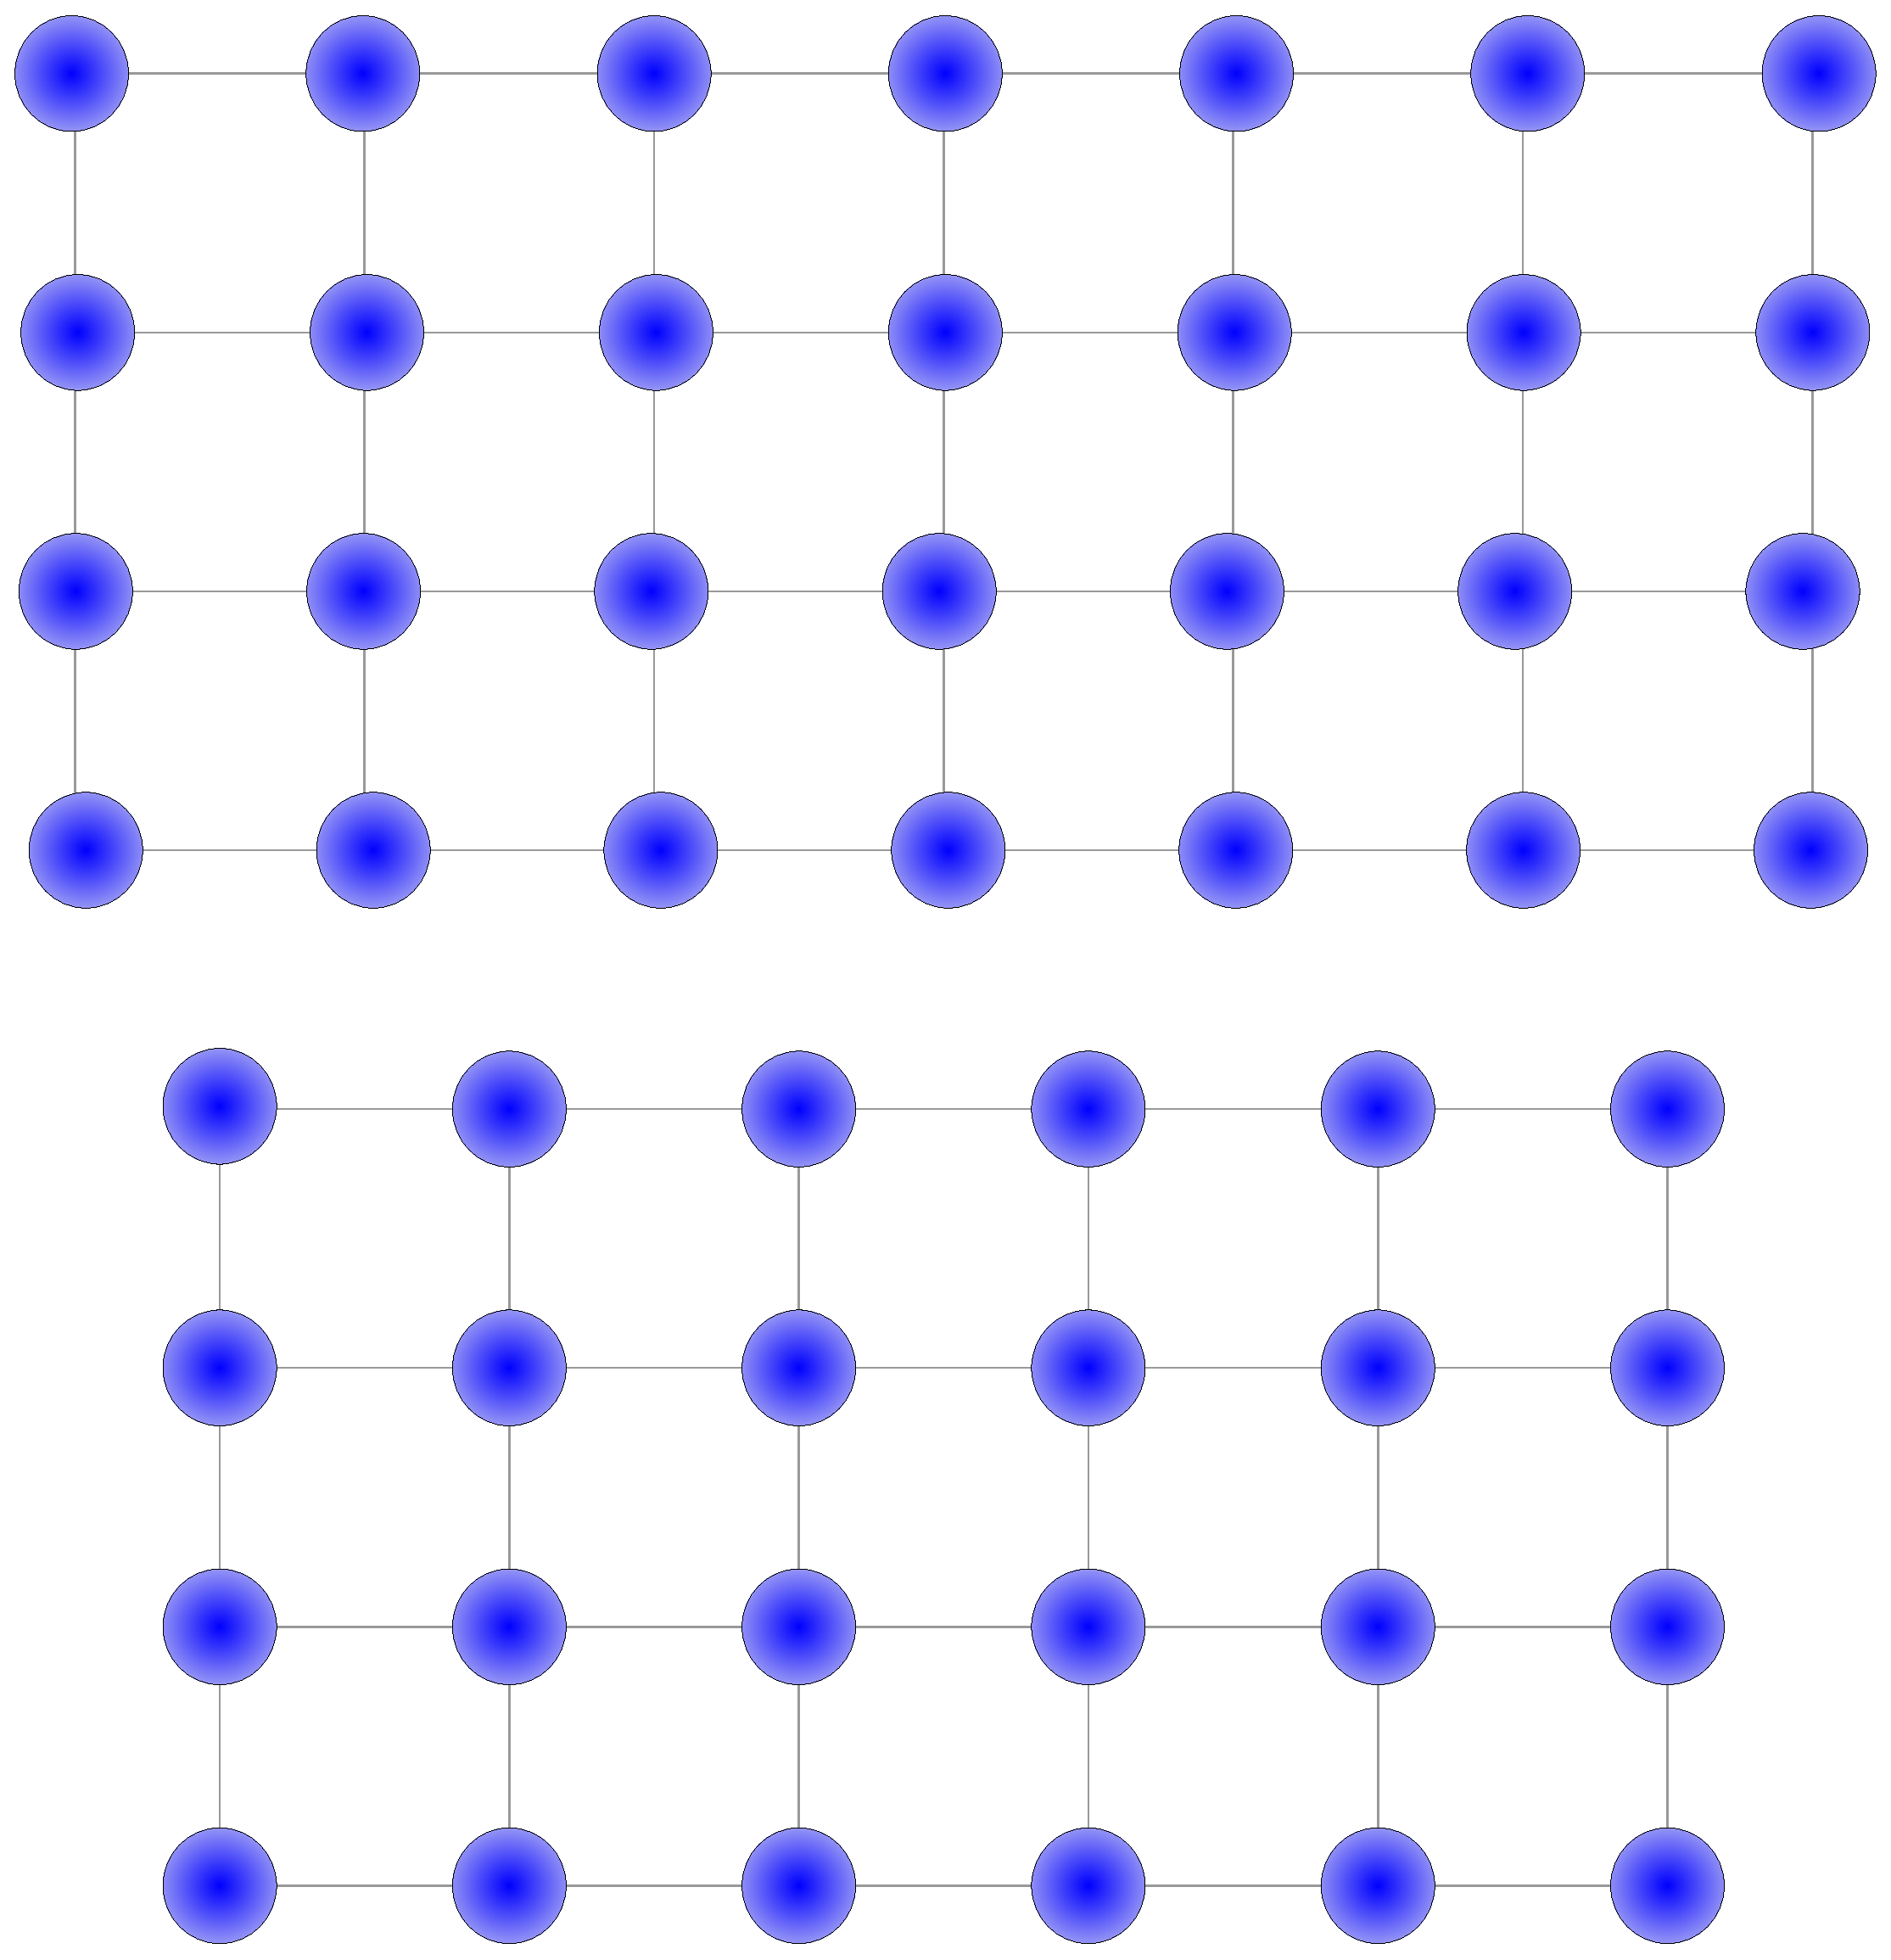
\includegraphics[width=\textwidth]{Half_crystals}
\caption{Two semi-infinite crystals misaligned by half of one Burgers vector. There is a planar defect between them.\label{fig:planar_defect}}
\end{subfigure}
~
\begin{subfigure}{0.35\textwidth}
\centering
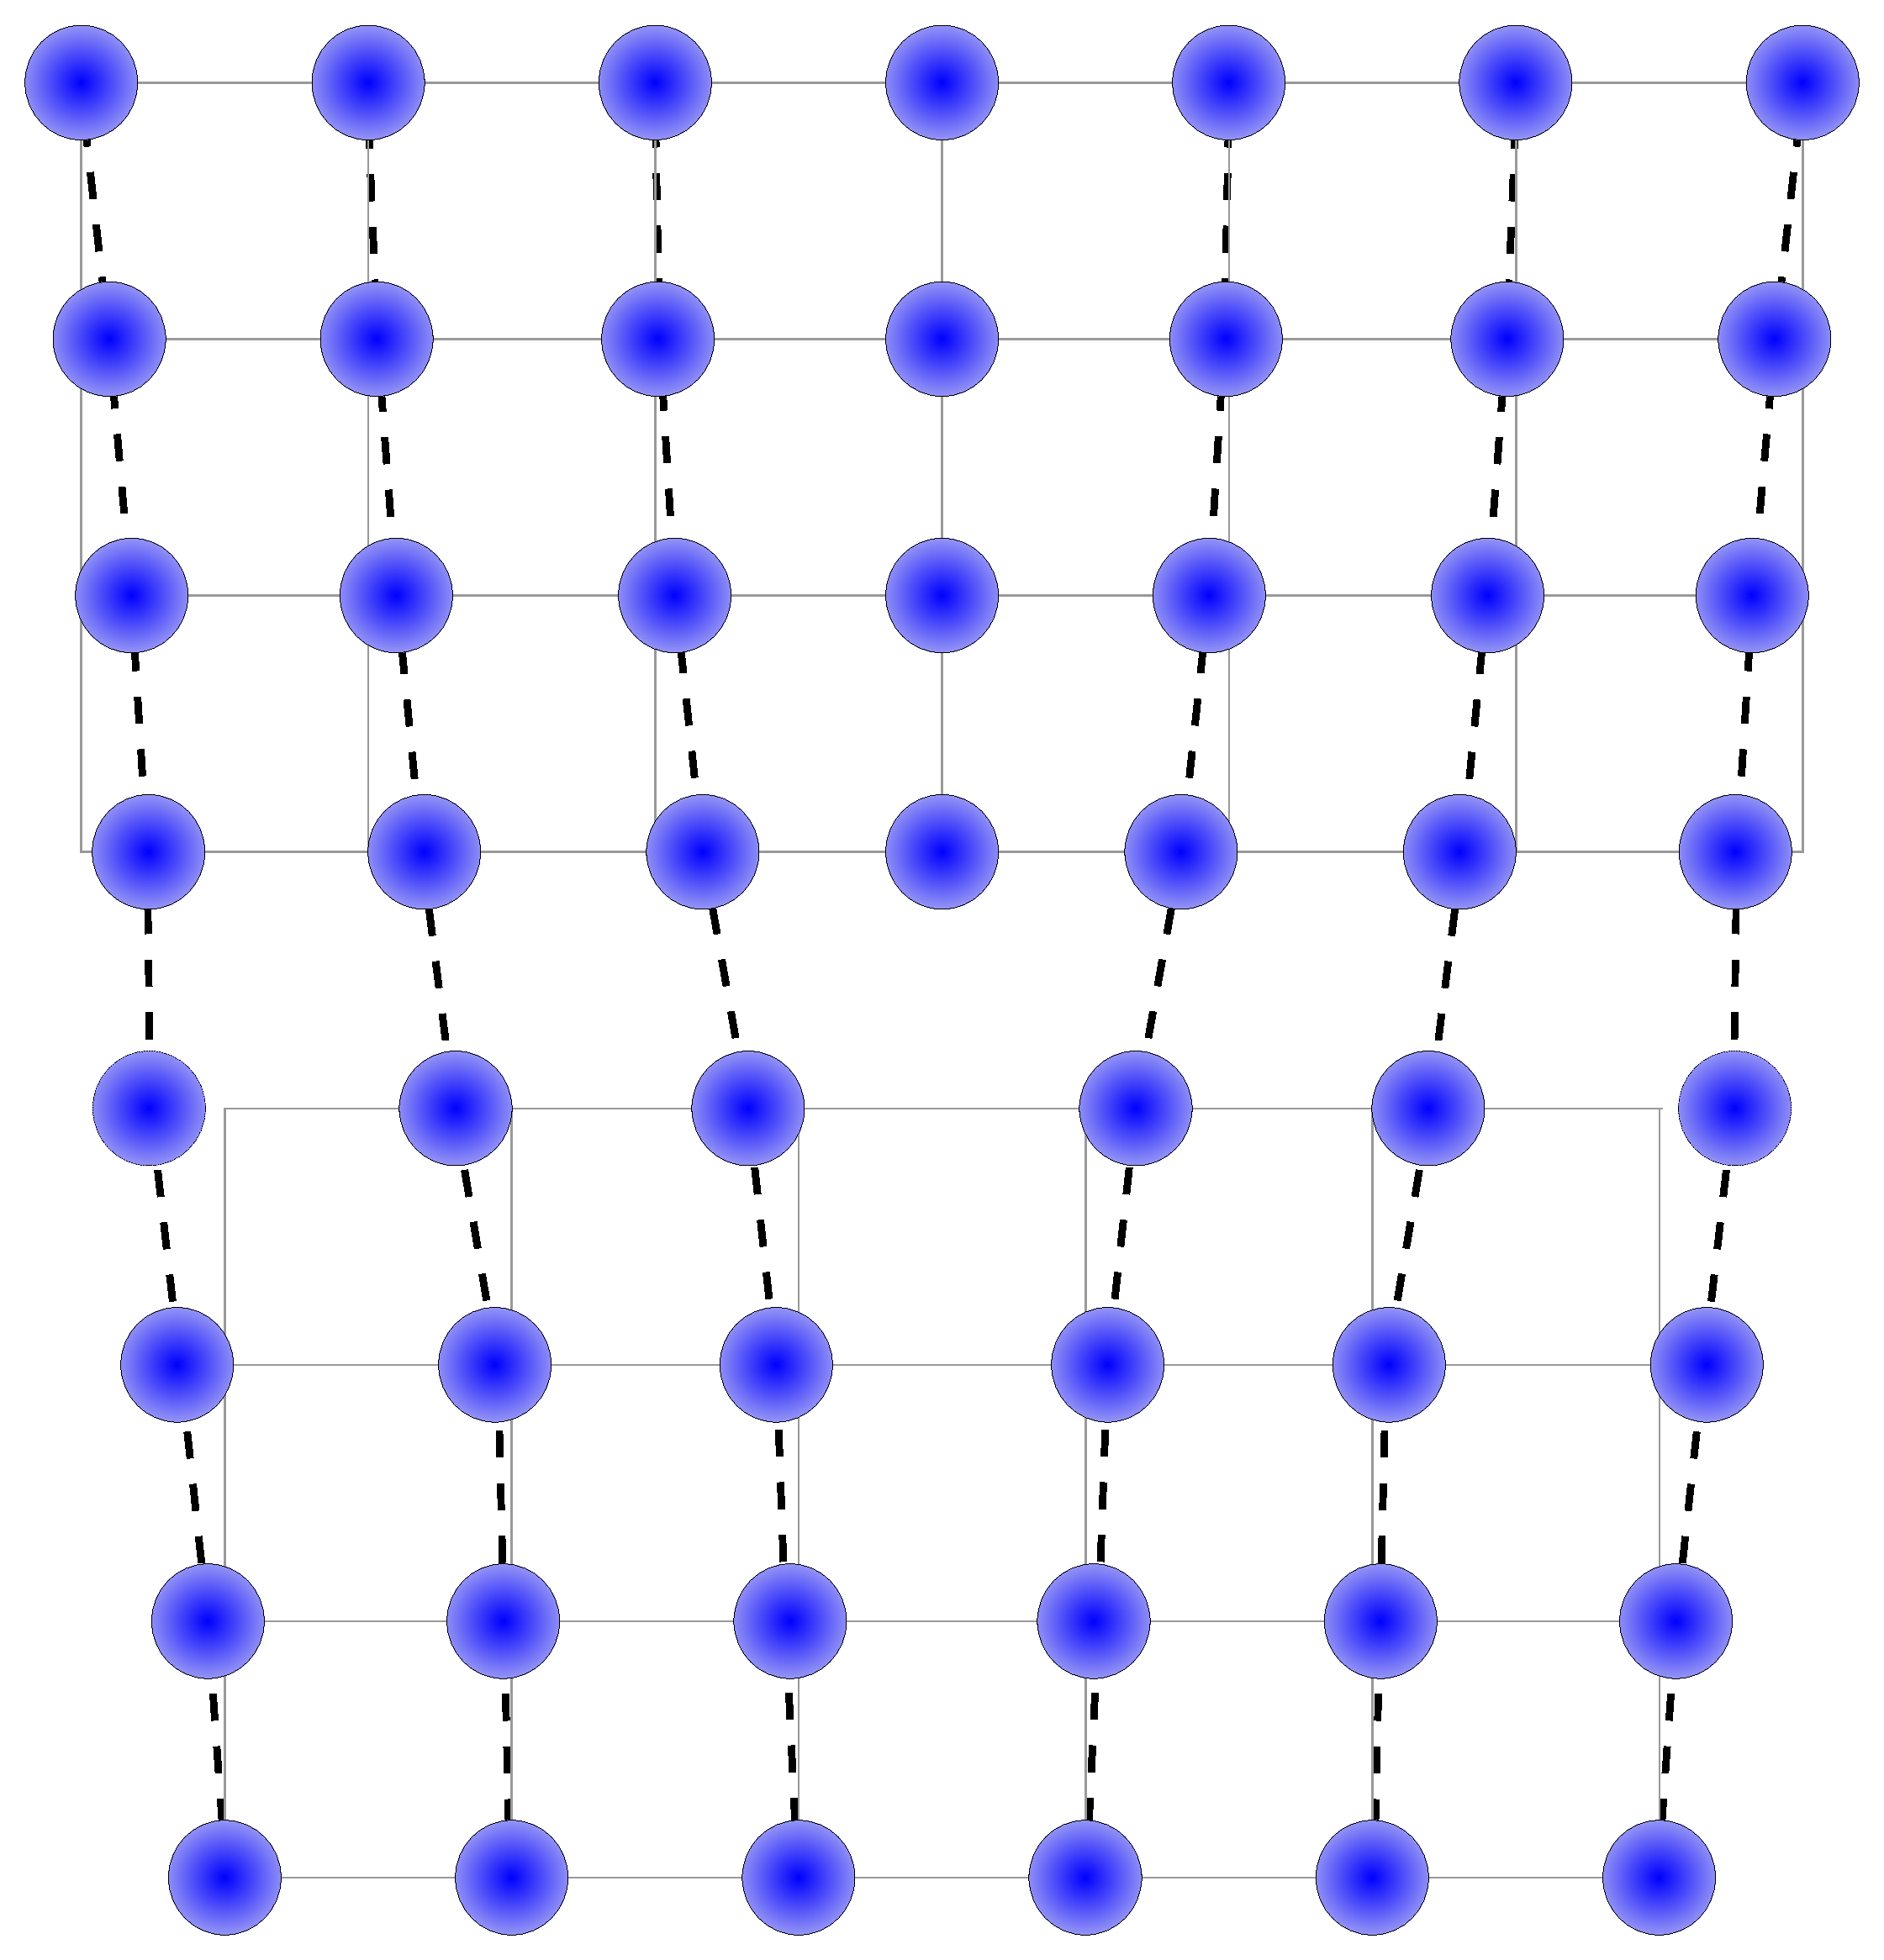
\includegraphics[width=\textwidth]{Edge_Dislocation_blank}
\caption{The atomic positions relax to form a dislocation, localising the strains and forming a linear defect.\label{fig:linear_defecct}}
\end{subfigure}
\caption{The formation of a dislocation, i.e.\ a line defect, from a planar defect.\label{fig:making_a_disloc}}
\end{figure}

\FloatBarrier
These two components favour different geometries of defect. In the case of the planar defect, the misalignment energy is at a maximum since the maximum number of cells are sheared the maximum amount, but the normal in-plane energy is at a minimum, in fact it's zero. In contrast localising the strains by aligning atoms across the slip plane will reduce the misalignment energy but increase the in-plane energy. The sum of these competing components will therefore pass through a minimum where the zone with large misalignments has a width that is neither zero or infinite. These two strain components, and the displacements that cause them are shown in \autoref{fig:peierls_details}.




\begin{figure}
\centering
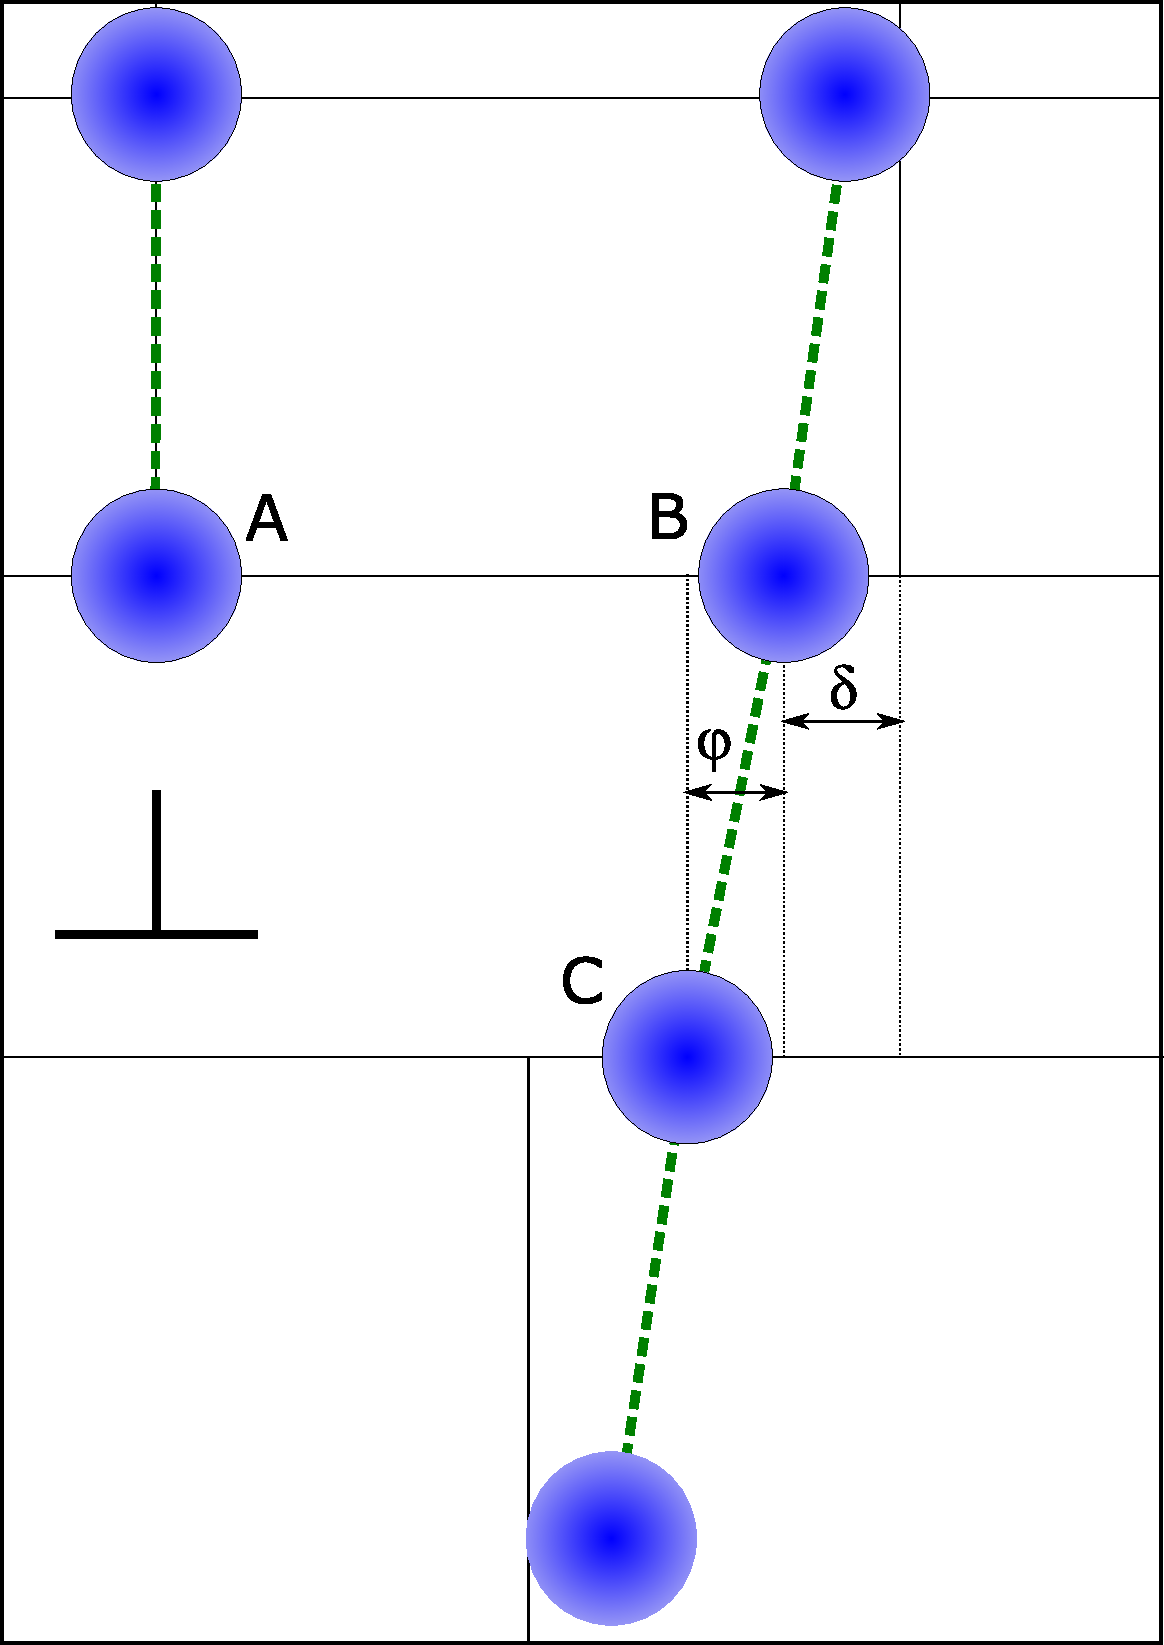
\includegraphics[width=0.5\textwidth]{peierls_model_detail}
\caption{The details of the relative displacements of atomic positions that give rise to strains around the core of a dislocation.\label{fig:peierls_details}}
\end{figure}

Using the displacements as defined in \autoref{fig:peierls_details}, and taking the equilibrium spacing to be $b$ parallel to the slip plane, and $d$ perpendicular to it, we can calculate the energy of the ``bonds''.

First the normal strains, caused by the displacement $\delta$, we can make the assumption that the energy is described by linear elasticity. Superficially this appears to imply that the energy should be $U_\text{i}=0.5E\varepsilon^2$. However this is not quite accurate, we need to account for the poisson strains, and any constraints on them.

\FloatBarrier
We start with the constitutive equations for an isotropic material (we'll make the assumption that the material is elastically isotropic for simplicity):

\begin{align*}
\varepsilon_1 = \frac{\sigma_1}{E} - \nu \frac{(\sigma_2 + \sigma_3)}{E} \\
\varepsilon_2 = \frac{\sigma_2}{E} - \nu \frac{(\sigma_1 + \sigma_3)}{E} \\
\varepsilon_3 = \frac{\sigma_3}{E} - \nu \frac{(\sigma_1 + \sigma_2)}{E} 
\end{align*}

I will define the 1, 2 and 3 directions relative to the edge dislocation such that the 1-axis is parallel to the Burgers vector, the 2-axis is parallel to the slip plane normal and the 3-axis is parallel to the line vector.


We can apply some boundary conditions to this situation. The symmetry of the dislocation line means there are now strains along the line, hence $\varepsilon_3 = 0$. We can also say that there is no physical reason to constrain the motion of atoms normal to the slip plane (at least as a first order approximation, neglecting the effect of strain gradients), so we can say that $\sigma_2 = 0$.

The former of these constraints gives us:
\begin{align*}
\frac{\sigma_3}{E} - \nu \frac{(\sigma_1 + \sigma_2)}{E} &= 0 \\
\sigma_3 - \nu \sigma_1 &= 0 \\
\sigma_3 &= \nu \sigma_1
\end{align*}

The positive sign here makes sense; the material would naturally contract (i.e.\ a negative strain) due to a perpendicular tension, but if constrained must be under a tension to oppose that effect.

Substituting back into $\varepsilon_1$:
\begin{align}
\varepsilon_1 &= \frac{\sigma_1}{E} - \nu \frac{(0 + \nu \sigma_1)}{E} \nonumber\\
&=\frac{\sigma_1 (1-\nu^2)}{E}\label{eqn:strain_one}
\end{align}

We can then use the equation for strain energy:
\begin{align*}
U &= \dfrac{1}{2} \varepsilon_i \sigma_i \qquad\begin{annotation}
\text{Note the summation convention over}\quad i=1,2,3 
\end{annotation}\\
U &= \dfrac{1}{2}(\varepsilon_1 \sigma_1 + \varepsilon_2 \sigma_2 + \varepsilon_3 \sigma_3)
\end{align*}

We know from the diagram in \autoref{fig:peierls_details} that $\varepsilon_1=\delta/b$ and since $\sigma_2=0$ and $\varepsilon_3=0$, we need only consider the first term. So rearranging \autoref{eqn:strain_one} and substituting for $\sigma_1$ we can write:
\begin{align}
U=\dfrac{1}{2} \varepsilon_1 \frac{E\varepsilon_1}{1-\nu^2} \nonumber\\
U= \frac{E}{2(1-\nu^2)}\varepsilon_1^2
\end{align}
This is in units of \si{\joule\per\meter^3}, if we want to consider the energy of a dislocation we must consider the energy per unit length, so we must multiply this volume energy by the area that lies perpendicular to the line length, i.e. $A= bd$, and substituting $\varepsilon_1 = \delta/b$:

\begin{equation}
U_{\text{line}} = \frac{E}{2(1-\nu^2)}\delta^2 \,\frac{d}{b}
\end{equation}

The energy of bonds misaligned across the slip plane are not so easily derived from first principles (albeit with some assumptions). Instead the best first approximation is not so much to make some assumptions as to take a large leap of faith. We assume that the small region of misaligned slip plane can be treated as a generalised planar fault. In IA the idea of stacking faults has been introduced, e.g.\ twinning in f.c.c. metals like Cu, or faults trailing a partial dislocation. 

These sorts of faults have generally have fixed offsets, for example in a ccp metal the usual stacking sequence is ...ABCABC... so a stacking fault might be ...ABCBA... where a plane that should be an A plane is a B plane, so there is a fixed misalignment equal to the displacement between those two sites. The concept can be generalised to a completely continuous misalignment from aligned through some sort of maximum misalignment and then returning to zero when the next site become aligned





\clearpage







\subsection{plasticity of isotropic materials}
The application of a tensile stress to an isotropic material produces perpendicular contraction stresses:
\begin{equation}
\varepsilon_{2} = \varepsilon_{3} = - \nu \varepsilon_{1}
\end{equation}
This gives the dilatation, or volume strain, as:
\begin{equation}
\Delta = \varepsilon_1 + \varepsilon_2 + \varepsilon_3 = \varepsilon_1 (1 - 2\nu)\label{eqn:volume_change_poisson}
\end{equation}
 
For most structural materials like metals, $\nu \approx 0.3$ and so for a strain of around \SI{0.5}{\percent} there is a volume change of around \SI{0.2}{\percent}. \autoref{eqn:volume_change_poisson} shows that as $\nu$ approaches 0.5 the volume change will approach zero.
 
However during plastic deformation there is no volume change

\section{Compressive Failure}

\subsection{Crushing}

You will be familiar with tensile failure from IA, that when the elastic energy released by growing a crack exceeds any work done in creating new surfaces or deforming material at the crack tip then catastrophic failure will occur. This is also intuitively reasonable since the stresses are acting to pull the atoms apart.

In contrast, it is not necessarily clear how a material will fail when the stresses act to push the atoms together. To understand why failure occurs we must consider the stress state more thoroughly.

\FloatBarrier
\begin{figure}[h!]
\centering
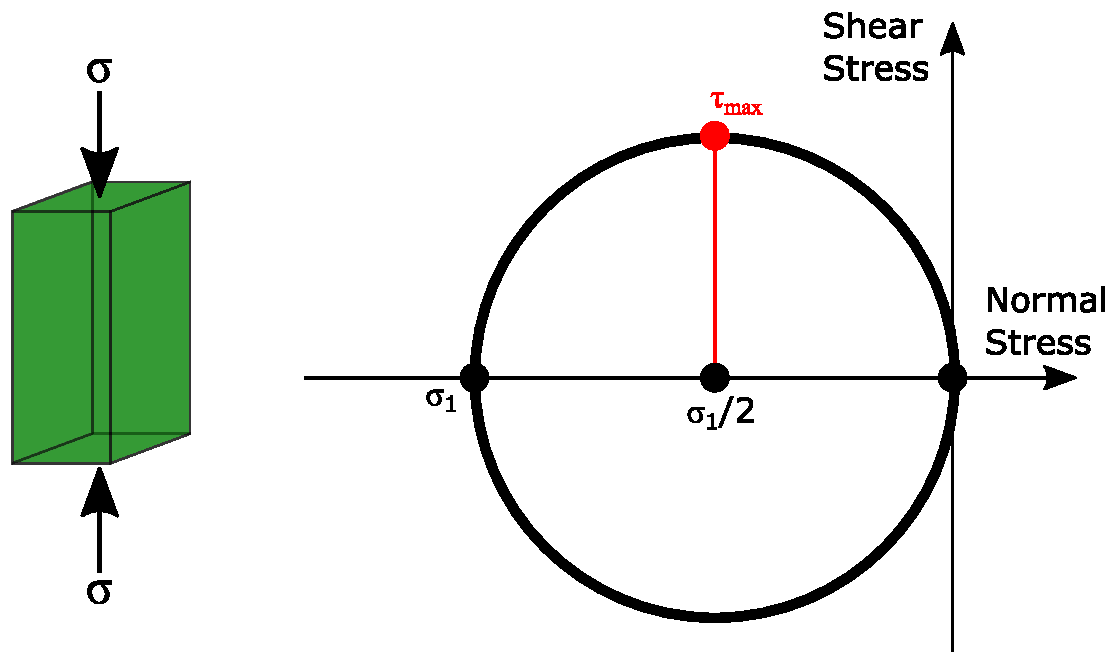
\includegraphics[width=0.6\textwidth]{compression_and_stress_state}
\caption{The stress state in a uniaxial compression test.\label{fig:compressive_stress_state}}
\end{figure}

\FloatBarrier

The Mohr's circle shown in \autoref{fig:compressive_stress_state} shows that there will be a shear stress in the material, that has a maximum value on planes inclined by \SI{45}{\degree} to the compression axis. There will be a driving force for crack growth along these planes:

\FloatBarrier
\begin{figure}
\centering
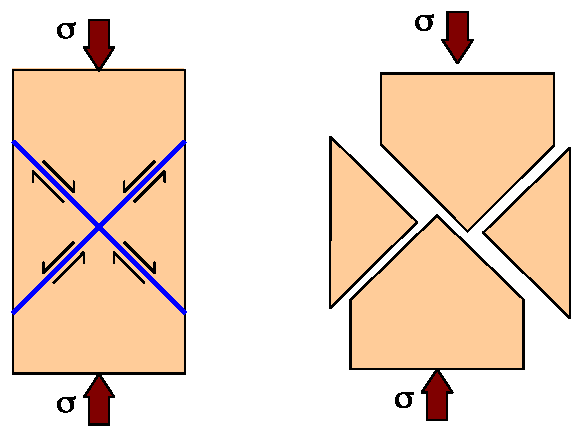
\includegraphics[width=0.7\textwidth]{crushing_schematic}
\caption{Schematic showing the way that shear stresses can give rise to a driving force for crack growth.}
\end{figure}

\FloatBarrier

\FloatBarrier
\begin{figure}[h!]
\centering
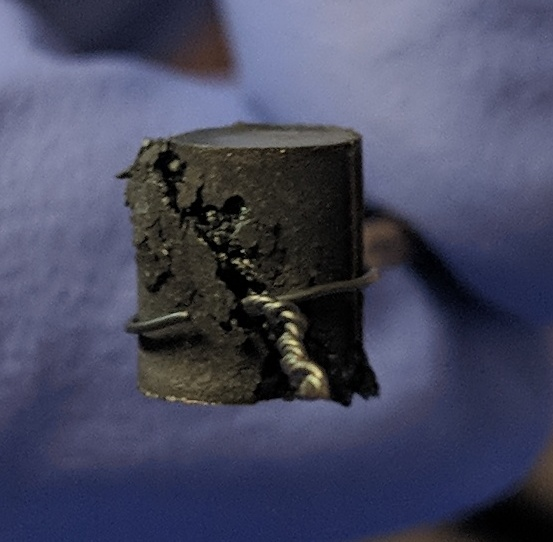
\includegraphics[width=0.5\textwidth]{crushed}
\caption{The failure of a nickel based superalloy compressed at \SI{1000}{\celsius}. The wire around the cylinder is a thermocouple to measure the temperature. With thanks to (soon to be Dr) Amy Goodfellow for the photograph.\label{fig:crushed}}
\end{figure}

\FloatBarrier



This is indeed seen in real materials, as shown in \autoref{fig:crushed}. Note that the crack seems to be intergranular, and runs across the sample at roughly \SI{45}{\degree}. The idealised case would have more than one single plane of failure, as shown in the schematic, but misalignment of the compression axis can add additional shear components to the stress state that favour one particular plane.

\subsection{Buckling}
\subsubsection{Elastic buckling}


Crushing of the material is only one of the ways that compressive failure may occur. If instead the elastic deformation of the material is large then this can lead to failure at loads lower than the crushing strength.

We will start by considering the compression of a freely hinged beam, i.e. the ends are on freely rotating pins, and the upper pin remains aligned vertically above the other:

\FloatBarrier
\begin{figure}[h!]
\centering
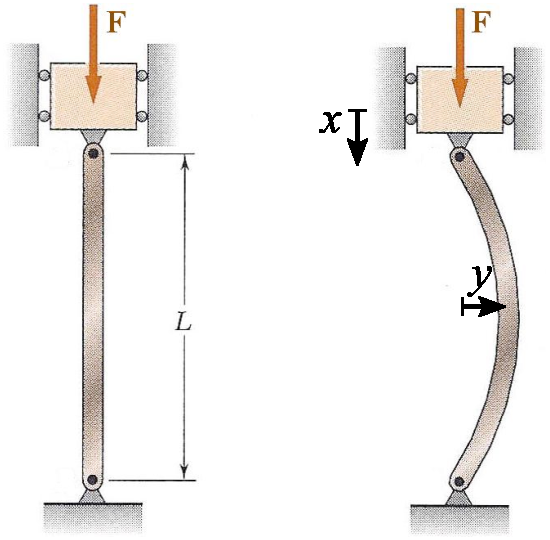
\includegraphics[width=0.6\textwidth]{freely_hinged_beam}
\caption{Compressive loading of a freely hinged beam that deflects elastically.\label{fig:free_hinge_deflection}}
\end{figure}
\FloatBarrier


In order to make this problem tractable we must assume a number of things:
\begin{enumerate}
\item The cross section is uniform. \begin{annotation} i.e.\ the beam doesn't taper. \end{annotation}
\item The material is homogeneous, isotropic and linear elastic.
\item The self weight (the forces due to the weight of the beam itself are negligible compared to the applied load.
\item The force is axial -- there is no eccentricity. \begin{annotation}  This is actually v.\ difficult to do in practice.\end{annotation}
\end{enumerate}

So considering the scenario shown in \autoref{fig:free_hinge_deflection}, there are two energy changes, firstly the work done by the applied force if the ends of the beam move:
\begin{equation}
\delta U_{\text{F}} = -F x \qquad\begin{annotation}
\text{-ve since the gpe of the system decreases.}
\end{annotation}
\end{equation}
\begin{annotation}
This energy change will favour buckling of the beam.
\end{annotation}

However the deflection of the beam will cause an internal energy change:
\begin{equation}
\begin{annotation}
\delta U_{\text{E}} > 0 \qquad \text{Energy is raised so opposes buckling.}
\end{annotation}
\end{equation}

This leads to a simple criterion as to whether buckling occurs or not:

\begin{equation}
\text{For buckling:} \qquad |\delta U_{\text{F}}| > |\delta U_{\text{E}}|
\end{equation}

If this is true the overall energy change will be negative and therefore favourable. To determine this we must consider the elastic energy of the beam, as a function of the displacement $y$.


If we consider a point along the beam, denoted $Q$, while the force applied is exactly equal to the critical load and the beam is in static equilibrium:
\FloatBarrier
\begin{figure}[h!]
\centering
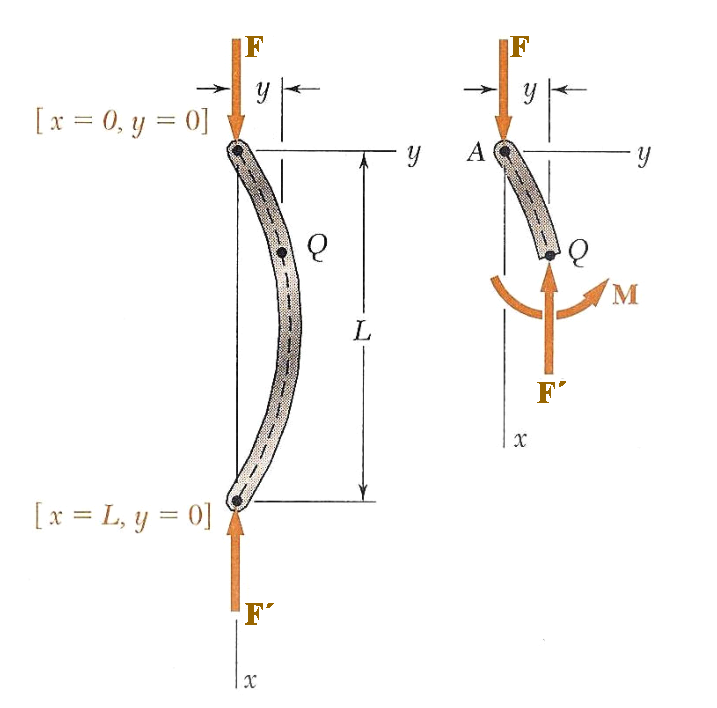
\includegraphics[width=0.5\textwidth]{moments_in_buckling}
\caption{}
\end{figure}
\FloatBarrier
We can say that the moment due to the external forces at the point $Q$ is:
\begin{equation}
M=-Fy
\end{equation}
which must be balanced by the internal moments generated by the stresses in the material. We can use the beam bending equation from earlier:
\begin{equation}
M=\kappa E I = \frac{d^2y}{dx^2}EI
\end{equation}

\begin{annotation}
Defining $ x$ and $y$ in this odd way ensures that these differential equations look the same.
\end{annotation}

These moments can be  set equal to each other:
\begin{equation}
-Fy = \frac{d^2y}{dx^2}EI \label{eqn:diff_equation}
\end{equation}
\begin{annotation}
\begin{equation}
\frac{d^2y}{dx^2} + \frac{Fy}{EI} = 0
\end{equation}
\end{annotation}

This is similar to the equation for beam bending, \autoref{eqn:beam_curvature}, but here the moment is also a function of the displacement, $y$, and the moment will increase as the deflection increases.

\autoref{eqn:diff_equation} is of the form:
\begin{equation}
\frac{d^2y}{dx^2} + k^2y = 0
\end{equation}
where $k=\frac{F}{EI}$, which is an ordinary second order differential equation and has a general solution of the form:
\begin{equation}
y = A\sin kx + B \cos kx
\end{equation}


The boundary conditions are that the ends of the beam remain aligned vertically, so that:

\begin{equation}
x=0, x=L \implies y = 0
\end{equation}

Using $y=0$ when $x=0$:
\begin{equation}
A \sin 0 + B \cos 0 = 0
\end{equation}
which implies that $B=0$. \begin{annotation} This leaves the form as a simple sine curve, $y=A\sin kx$ \end{annotation}
\\

Then using $y=0$ when $x=L$:
\begin{equation}
A \sin kL = 0
\end{equation}
One simple solution to this is that $A=0$, however this is simply the case when the beam has not deflected at all and therefore can be discounted. If $A \neq 0$ then:
\begin{align}
\sin kL = 0 \\
\implies kL = n\pi \qquad \text{where} \,\, n \,\, \text{is an integer.}\nonumber
\end{align}

Recalling that $k^2 = F/EI$ we can write that:
\begin{equation}
\frac{F_{\text{EB}}}{EI} = \frac{n^2\pi^2}{L^2}
\end{equation}
and therefore finally the force required for elastic buckling is given by:
\begin{equation}
F_{\text{EB}} = \frac{n^2 \pi^2 EI}{L^2}
\end{equation}

This gives rise to the possibility of more than one configuration of buckling since $n$ can take any integer value, as shown in \autoref{fig:buckling_configs}. However, since the force required for each mode increases with $|n|$ the beam will fail by buckling with $n=\pm1$, and $|n|>1$ will not occur unless further constraints are placed on the beam.

\begin{figure}
\centering
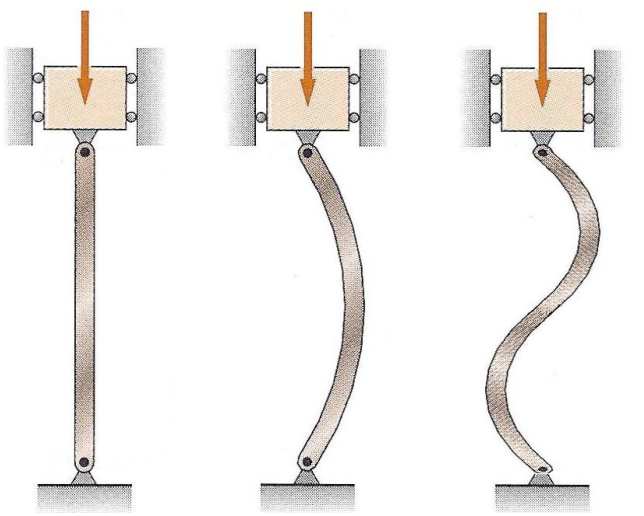
\includegraphics[]{buckling_configs}
\caption{Possible configurations of the elastic buckling of a beam. Those with $n > 1$ are of no practical interest.\label{fig:buckling_configs}}
\end{figure}

For forces lower than this any perturbation sideways will raise the energy of the system and the beam will straighten itself to lower the elastic energy, and hence will not buckle. When $F=F_{\text{EB}}$ static equilibrium in the $n=\pm1$ configuration is achieved, and if the force exceeds this then the column becomes unstable and the beam will fail catastrophically as soon as it is perturbed from perfectly straight


The failure stress of a column, by elastic buckling is therefore:
\begin{equation}
F_{\text{EB}} = \frac{\pi^2 EI}{L^2}
\end{equation}

This represents an upper bound on the failure load of a beam, since defects in the material such as inhomogeneity or pores/dimensional variations could cause the true value to be lower. It's also unlikely that the loading will be purely axial and this would also lower the failure load.

\subsubsection{The effects of end constraints}

Many real scenarios will not have freely rotating ends but instead will have fixed or clamped ends. First let's consider the case of one end clamped and one end free to rotate:
\FloatBarrier
\begin{figure}[h!]
\centering
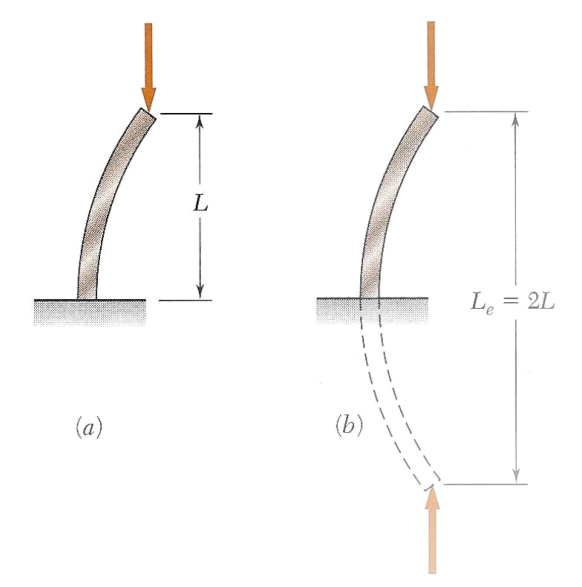
\includegraphics[width=0.5\textwidth]{one_fixed_one_free}
\caption{The buckling load of a beam with one fixed end can be easily calculated by considering an ``effective length''.   }

\begin{annotation}
The length $2L$ is equivalent to the $L$ used in the derivation for two free ends. 
\end{annotation}
\end{figure}
\FloatBarrier

By using the ``effective length'' the elastic buckling force is:
\begin{equation}
F_{\text{EB}} = \frac{\pi^2EI}{(2L)^2} = \frac{1}{4}\frac{\pi^2EI}{L^2}
\end{equation}
\begin{annotation}
The failure load has been reduced by a factor of 4.
\end{annotation}

The other likely scenario is when both ends are fixed, and a similar approach is possible:
\FloatBarrier
\begin{figure}[h!]
\centering
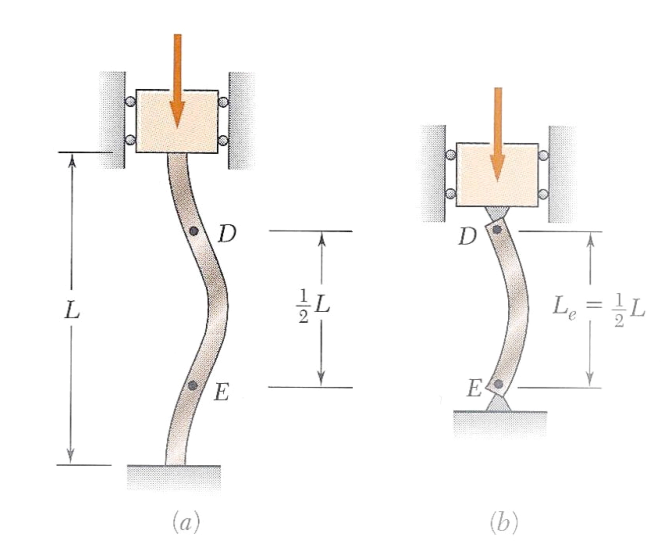
\includegraphics[]{two_fixed_ends}
\caption{The radius of curvature has decreased, and the new shape has an effective length of $L/2$.}
\end{figure}
\FloatBarrier

This alters the force required for elastic buckling to be:
\begin{equation}
\begin{annotation}
F_{\text{EB}} = \frac{\pi^2EI}{(L/2)^2} = 4 \frac{\pi^2EI}{L^2}
\end{annotation}
\end{equation}

\begin{quotation}
The buckling load has increased by a factor of 4.
\end{quotation}


We can write a final expression where the nature of the ends of the beam are included as a constant:
\begin{equation}
F_{\text{EB}} = c \frac{\pi^2 EI}{L^2}
\end{equation}
where $c$ may take a value of $^1\!/_4$, $1$ or $4$ depending on the situation in question.


\subsubsection{The effect of aspect ratio}

We can write an expression for the stress in a beam when elastic buckling occurs:
\begin{equation}
\sigma_{\text{EB}} = \frac{F_{\text{EB}}}{A} = c \frac{\pi^2 E I }{L^2 A}
\end{equation}
and assuming that we have a cylindrical beam we can link $I$ and $A$ to the radius, $R$:
\begin{equation}
\begin{annotation}
I = \frac{\pi R^4}{4} \qquad \qquad A= \pi R^2
\end{annotation}
\end{equation}
and substituting these in:
\begin{equation}
\sigma_{\text{EB}} = \frac{c}{4} \frac{\pi^2 E}{(L/R)^2}
\end{equation}

Thus the stress at which a beam will buckle depends on the aspect ratio. This is perhaps familiar from every day life, that as a beam becomes longer and more slender the stress required for it to fail by elastic buckling decreases.

The ratio $L/R$ is called the slenderness ratio and is the crucial geometric factor in the failure of a beam. The only material property that affects the the buckling stress of a beam is the Young's modulus $E$. These two effects can be represented graphically:

\FloatBarrier
\begin{figure}[h!]
\centering
\begingroup%
  \makeatletter%
  \providecommand\color[2][]{%
    \errmessage{(Inkscape) Color is used for the text in Inkscape, but the package 'color.sty' is not loaded}%
    \renewcommand\color[2][]{}%
  }%
  \providecommand\transparent[1]{%
    \errmessage{(Inkscape) Transparency is used (non-zero) for the text in Inkscape, but the package 'transparent.sty' is not loaded}%
    \renewcommand\transparent[1]{}%
  }%
  \providecommand\rotatebox[2]{#2}%
  \ifx\svgwidth\undefined%
    \setlength{\unitlength}{397.00601893bp}%
    \ifx\svgscale\undefined%
      \relax%
    \else%
      \setlength{\unitlength}{\unitlength * \real{\svgscale}}%
    \fi%
  \else%
    \setlength{\unitlength}{\svgwidth}%
  \fi%
  \global\let\svgwidth\undefined%
  \global\let\svgscale\undefined%
  \makeatother%
  \begin{picture}(1,0.55617582)%
  \begin{annotation}
    \put(0,0){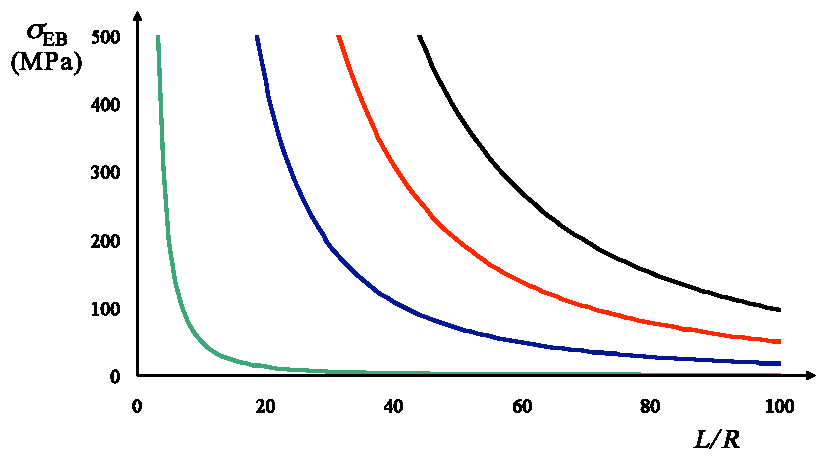
\includegraphics[width=\unitlength,page=1]{slenderness_buckling.pdf}}%
    \put(0.32520198,0.52828452){\makebox(0,0)[lb]{\smash{For \textit{c}=1}}}%
    \put(0.34476807,0.1194207){\makebox(0,0)[lb]{\smash{Nylon}}}%
    \put(0.55678051,0.16588762){\makebox(0,0)[lb]{\smash{Al}}}%
    \put(0.68741711,0.19937701){\makebox(0,0)[lb]{\smash{Fe}}}%
    \put(0.79951108,0.23074506){\makebox(0,0)[lb]{\smash{\ce{Al2O3}}}}%
    \put(0,0){\includegraphics[width=\unitlength,page=2]{slenderness_buckling.pdf}}%
    \put(0.7158491,0.52){\makebox(0,0)[lb]{\smash{Increasing Stiffness}}}%
    \put(0.7158491,0.48){\makebox(0,0)[lb]{\smash{Buckling is less likely}}}%
    \put(0.7158491,0.44){\makebox(0,0)[lb]{\smash{Survive higher stress}}}%
    \put(0.7158491,0.40){\makebox(0,0)[lb]{\smash{Or higher slenderness}}}%
    \end{annotation}
  \end{picture}%
\endgroup%
\caption{The variation of the buckling stress with slenderness ratio for a number of different material stiffnesses}
\end{figure}
\FloatBarrier

\subsubsection{The effect of cross-section shape}

As we know from IA and have recapped earlier in the course, the shape of a beam's cross-section is important when considering the deflection of the beam, this is quantified by the second moment of area, $I$. In a horizontal beam we already know which way the moment will be applied and this leads to the I-beam we are familiar with. However in buckling the beam might deflect in any direction and so is most likely to deflect such that $EI$, the beam stiffness, is smallest, and since $E$ usually doesn't vary this means the direction for which $I$ is smallest.

\FloatBarrier

\begin{figure}[h!t]
\centering
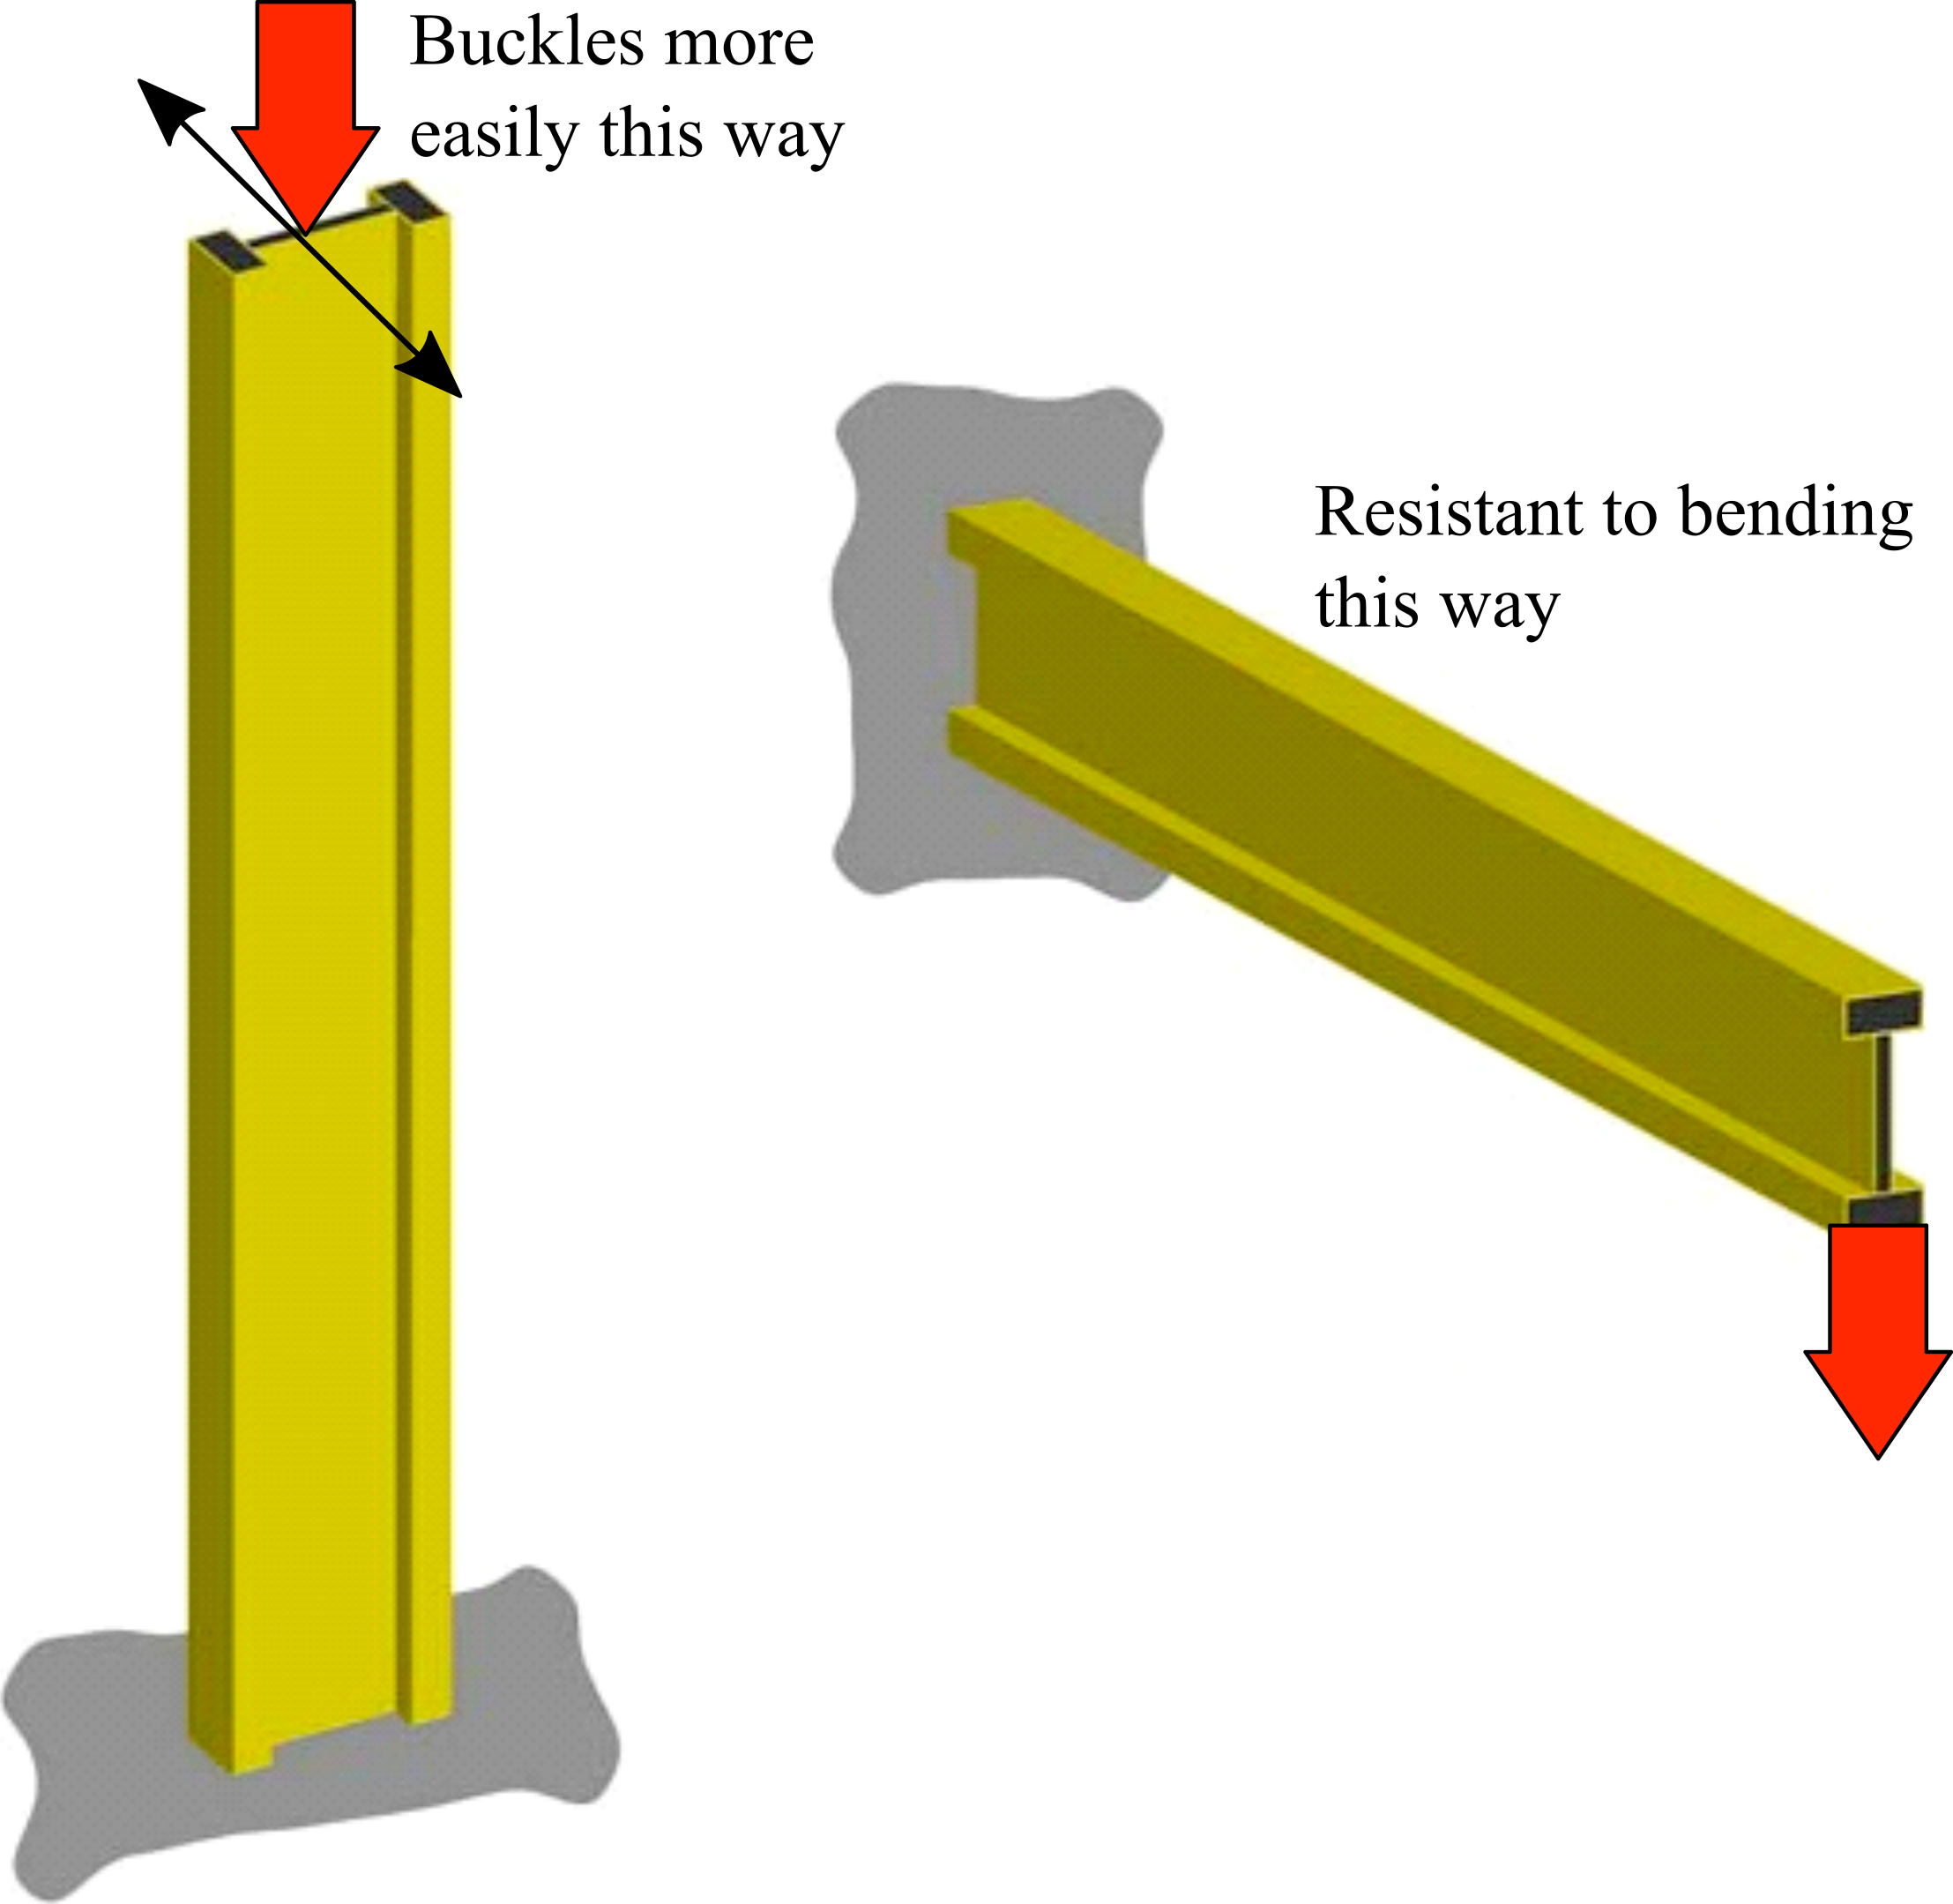
\includegraphics[width=9cm]{I_beam}
\end{figure}
\FloatBarrier


For this reason there is little benefit to shapes such as I-beams, and instead a cylindrical cross sections, or other rotationally symmetric shapes (squares, equilateral triangles etc.), are best (for a given column height and a given volume of material).

This leads to a way in which the volume (and therefore the cost) of material can be kept constant, while increasing the second moment of area. A hollow cross section will result in moving material away from the neutral axis and so increase $I$, and increase the resistance to buckling.

\FloatBarrier
\begin{figure}[h!b]
    \centering
    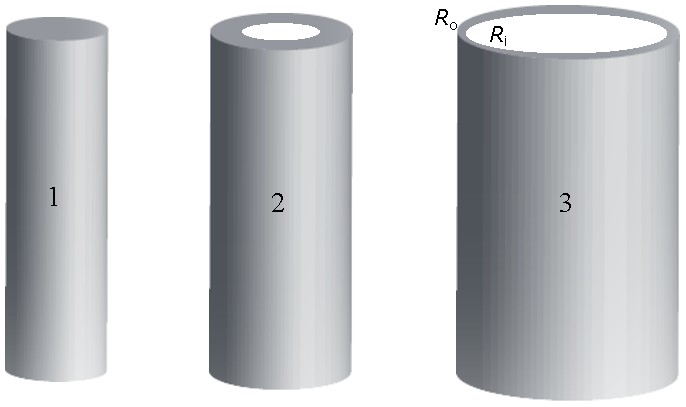
\includegraphics[width=0.6\textwidth]{hollow_cylinders}
    \caption{Increasing the second moment of area by using a hollow cylinder (for a given volume of material). The greater the radius, the greater the resistance to elastic buckling.\label{fig:my_label}}
\end{figure}

The second moment of area for a hollow cylinder is given by:

\begin{equation}
    \begin{annotation}
    I = \frac{\pi (R_{\text{o}}^4 - R_{\text{i}}^4)}{4}
    \end{annotation}
\end{equation}
\begin{annotation}
Therefore $I_3 > I_2 > I_1$
\end{annotation}

Hence the use of hollow cylinders to mount road signs or build scaffolding.

\subsubsection{Does elastic buckling cause failure?}

Elastic buckling thus far has been described in purely elastic, and therefore reversible and recoverable, terms. However the change in shape usually leads to other forms of failure, such as brittle fracture in the regions of material under tensile stress, plastic deformation in either tension or compression, or local buckling may occur (we will discuss this shortly).

Reaching failure or not often depends on the loading scenario. Consider a test performed under {\bf displacement control}, in which we apply sufficient force to the end plates of a column to control the distance between them. Initially there will be simple elastic deformation of the material, but soon the buckling force is reached. However, the buckling will not lead to catastrophic collapse because as the force resisting the motion of the end plates drops, so too does the applied force. Instead the buckling will advance in a stable manner and can be reversed unless some other material failure has occurred.

\begin{annotation}
The load is not free to lower the energy of the system after $F_{\text{EB}}$ has been reached, instead the applied force is reduced to maintain a fixed displacement.
\end{annotation}

Alternatively a column may be tested under {\bf load control}. This is achieved by gradually increasing the load and measuring the displacement that arises (the simplest form of load control would be to stack weights on top of a column). Recalling the buckling will occur when the energy changes driving it exceeds the energy changes resisting it. This means that buckling will be sudden and the ends of the column will come together. If the material can recover from large strains, e.g.\ a rubber, then the column may recover when the load is reduced, but otheriwse will likely have failed due to large stresses and strains that develop in the beam.

\begin{annotation}
The load is free to continue doing work and lower the energy of the system, leading to complete failure.
\end{annotation}

\subsection{Local Buckling}

If we assume that elastic buckling is the only mode of failure that can occur (below an upper bound on the strength which is the ordinary compressive strength of the material) then this leads us to the conclusion that failure of the structure can be avoided simply by increasing the radius of a hollow cylindrical column, without increasing the amount of material.

Howver as the radius of the cross section increases the wall thickness must decrease (assuming a constant volume of material). There is a lower limit to the wall thickness that can be used, and below a critical thickness failure will occur by {\bf local buckling}. A paper straw crumpling is an example of this, and unlike elastic buckling, is always irreversible.

The force required for local buckling is given by:
\begin{equation}
    F_{\text{lb}} = k\pi E t^2
\end{equation}
where $t$ is the wall thickness, $E$ is the Young's modulus and $k \approx 0.5$ is a constant that depends of the surface imperfections. 

A drinks can is a good example of a structure that we know will fail by local buckling. We can calculate the force required for failure:

\begin{annotation}
\begin{figure}[t!]
    \centering
    
\includegraphics{generic_drink}
\end{figure}
\FloatBarrier

$$
t \approx \SI{100}{\micro\meter} \qquad \text{and Al:} \qquad E \approx \SI{70}{\giga\pascal}
$$

$$ F = 0.5  \pi ( 70\times 10^9 )(100\times 10^{-6})^2\approx \SI{1.1}{\kilo\newton} $$

$$\implies \sigma = \SI{50}{\mega\pascal}$$
\end{annotation}

\subsubsection{The effect of internal pressure}

\FloatBarrier
\begin{figure}[h!]
    \centering
    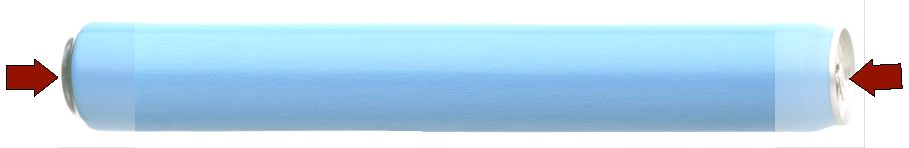
\includegraphics[width=\textwidth]{long_can}
\end{figure}
\FloatBarrier







\FloatBarrier
\clearpage
\printbibliography

\end{document}